% !TeX TXS-program:compile = txs:///pdflatex/[--shell-escape]
% =========================================================================
\documentclass[aspectratio=1610]{beamer}
%\documentclass[aspectratio=1610]{beamer}

% ========================= Theme =========================================
\usetheme{Berkeley}
\usecolortheme{seahorse}

% ========================= Essential packages ============================
%\usepackage{hyperref}
%\hypersetup{
%    colorlinks = true,
%    linkcolor = blue,
%    citecolor = blue,
%    filecolor = blue,
%    urlcolor = blue
%}

% ========================= Frame notes systm ============================
%\usepackage{pgfpages}
%\setbeameroption{show notes on second screen}

% ========================= Plotting ======================================
\usepackage{calc}
\usepackage{tikz}
\usetikzlibrary{arrows,
                arrows.meta,
                calc,
                chains,
                quotes,
                positioning,
                shapes,
                shapes.geometric}
\usepackage{graphicx}
\usepackage{graphics}
\usepackage{pgfplots}
\pgfplotsset{width=7cm,compat=1.17}

%% ============================== Tabular =================================
\usepackage{booktabs}
\usepackage{tabularx,ragged2e}
\usepackage{array}
\usepackage{multirow}
\usepackage{siunitx}
  \sisetup{detect-all}
\usepackage{adjustbox}
\usepackage{rotating}
\usepackage{threeparttable}
\usepackage[justification=centering]{caption}

%% ============================== Text boxes ==============================
\usepackage[most]{tcolorbox}		

%% ========================== Coding snippets =============================
% Default fixed font does not support bold face
%\usepackage{minted}
%\usemintedstyle{vs}

% ========================= Infor on authors ==============================
\title[Visualization Design]%
{Visualization Design}
\subtitle{Design Principles and Main Visual Forms}
\author{S.~Santoni\inst{1}}
\institute{
	\inst{1}%
	Bayes Business School
	}
\date{MSc in Business Analytics, 2024/25}

% ============================ Colors =====================================
\definecolor{base_c}{rgb}{0.6,0,0}
\definecolor{comp_c}{rgb}{0.09803921568627451, 0.6901960784313725, 0.7529411764705882}
\definecolor{tri_1}{rgb}{0.09803921568627451, 0.7686274509803922, 0.19215686274509805}
\definecolor{tri_2}{rgb}{0.19215686274509805, 0.09803921568627451, 0.7686274509803922}

% ========================= TOC  ==========================================
\AtBeginSection[]
{
	\begin{frame}
		       \frametitle{Outline}
		       \tableofcontents[currentsection,currentsubsection]
	\end{frame}
}

% ========================= References ===================================
\usepackage[style=numeric,backend=biber]{biblatex}
\addbibresource{bibliography.bib}

% =========================== TOC =========================================
\AtBeginSubsection[]
{
    \begin{frame}
        \frametitle{Outline}
        \tableofcontents[currentsection,currentsubsection]
    \end{frame}
}

% ========================= Document  ====================================
\begin{document}

\begin{frame}
	\titlepage
\end{frame}

\begin{frame}{Outline}
	\tableofcontents
\end{frame}

% ========================= Week 2 wrap up =================================
\section{Session \#2 Wrap Up}

\begin{frame}
	\frametitle{Graphical Excellence according to Tufte}
	Per Tufte's work \cite{tufte2001}, excellence in statistical graphs consists of complex
	\emph{``ideas communicated with clarity, precision, and
		efficiency.''}

	\vspace{1em}

	Graphical displays pursuing clarity, precision, and efficiency \emph{``
		give to the viewer the greatest number of ideas
		in the shortest time with the least ink in the smallest space.''}

	\begin{figure}
		\begin{small}
			\begin{center}
				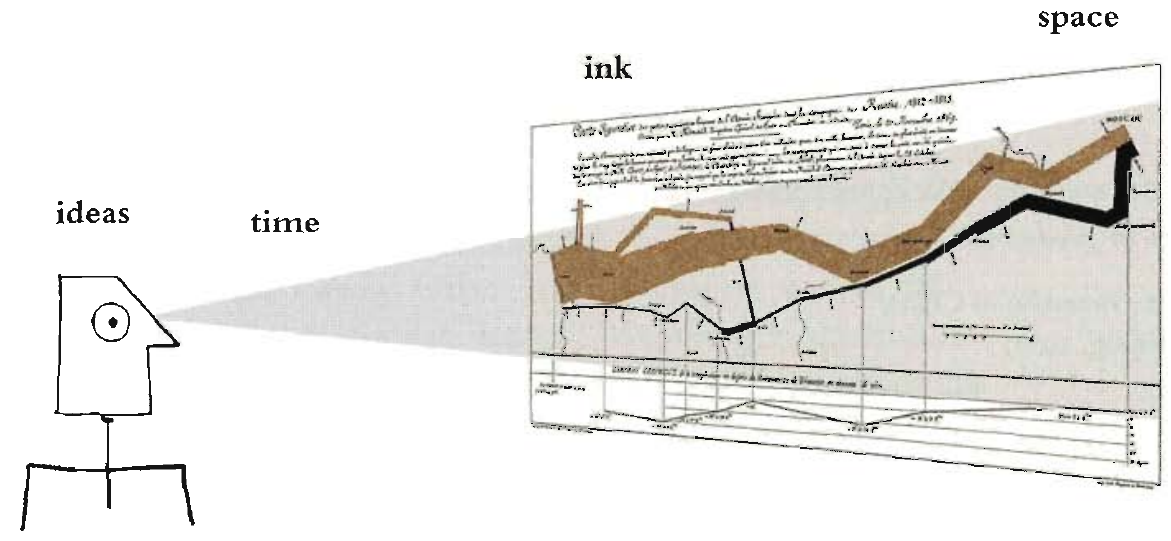
\includegraphics[width=0.75\textwidth]{
					images/graphical_excellence.png
				}
			\end{center}
		\end{small}
	\end{figure}
\end{frame}

\begin{frame}
	\frametitle{How to Reach Clarity, Efficiency, and Precision?}
	Tufte points out graphical displays should
	\begin{itemize}
		\item
		      Show the data
		\item
		      Induce the viewer to think about the substance rather than
		      about the methodology, graphical design, the technology of
		      graphic production, or something else
		\item
		      Avoid distorting what the data have to say
		\item
		      Present many numbers in a small space
		\item
		      Make large datasets coherent
		\item
		      Encourage the eye to compare different pieces of data
		\item
		      Reveal the data at several levels of detail, from a broad
		      overview to the fine structure
		\item
		      Serve a reasonably clear purpose: description,
		      exploration, tabulation, or decoration
		\item
		      Be closely intergrated with the statistical and verbal
		      description of a data set
	\end{itemize}
\end{frame}

\begin{frame}
	\frametitle{Yet another Time Series that Lies}
	\begin{figure}
		\begin{small}
			\begin{center}
				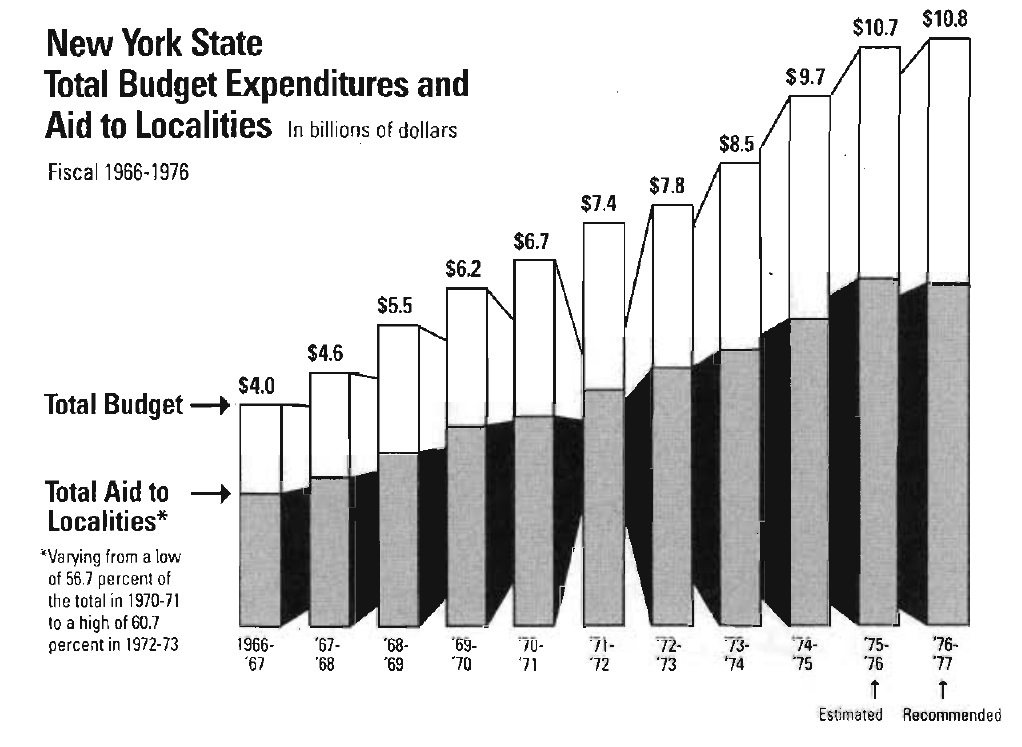
\includegraphics[width=0.7\textwidth]{
					images/nys_budget.png
				}
			\end{center}
		\end{small}
	\end{figure}

	\footnotesize
	Source: New York Times, February 1, 1976, page IV-6.
\end{frame}

\begin{frame}
	\frametitle{Let Us Redesign the `NYS Total Budget Expenditures' Graph}
	\begin{figure}
		\begin{small}
			\begin{center}
				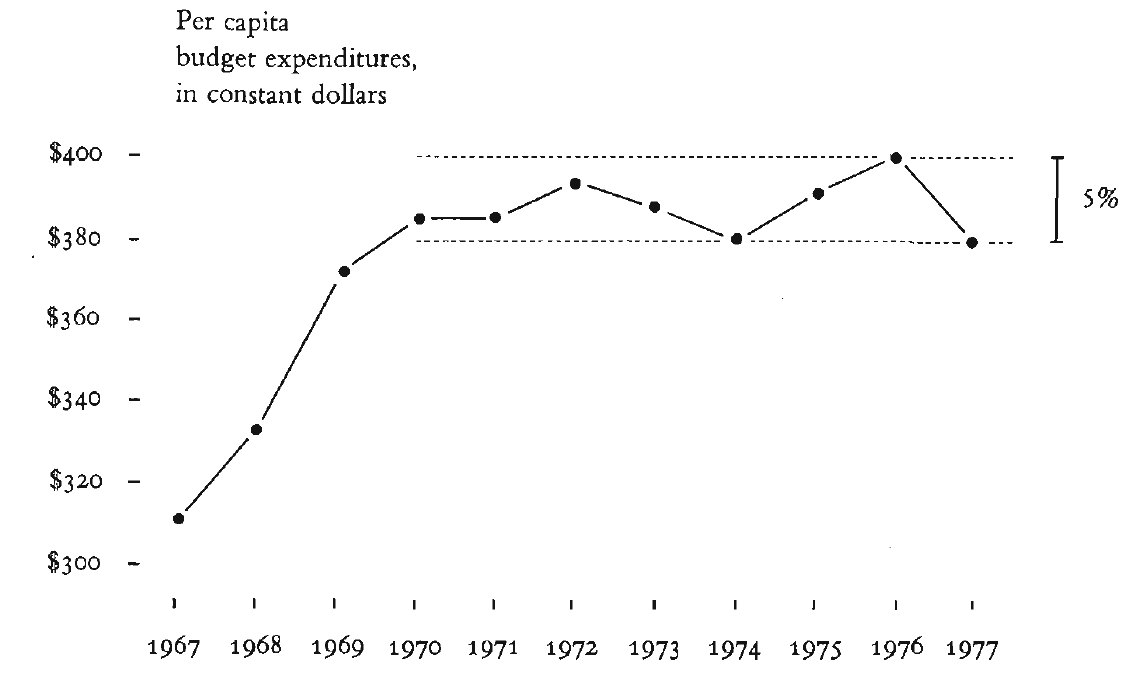
\includegraphics[width=0.8\textwidth]{
					images/redo_nys_budget.png
				}
			\end{center}
		\end{small}
	\end{figure}
\end{frame}

\begin{frame}{}
	\LARGE \centering Your version of Tufte's chart
\end{frame}

% =========================== Design principles ============================
\section{Design Principles}

\begin{frame}{The Data Visualization Process acccording to Cairo}
	{Data, information, knowledge, wisdom}{}
	\begin{figure}
		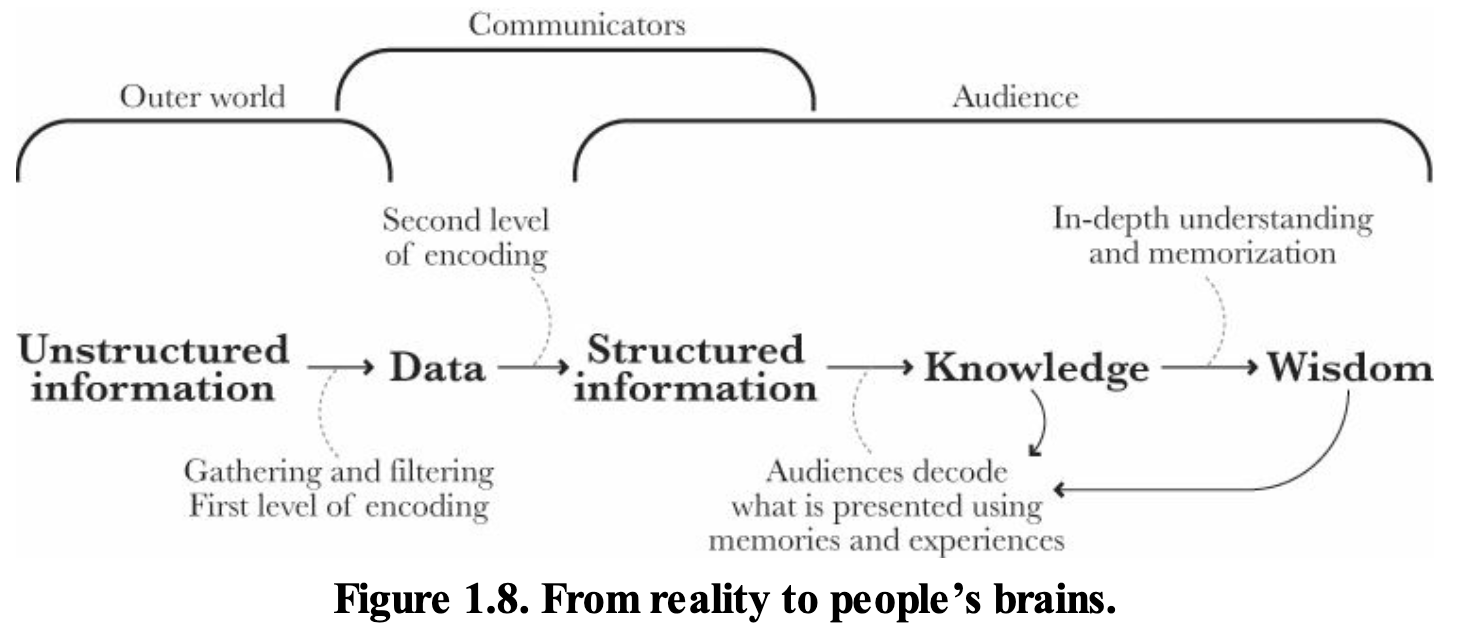
\includegraphics[width=0.95\textwidth]{images/cairo_model.png}
		\caption*{Source is \cite[][page 29]{cairo2012}}
	\end{figure}
\end{frame}

\begin{frame}{How to Navigate the Data Visualization Process?}
	\begin{columns}
		\begin{column}{0.5\textwidth}
			\begin{figure}
				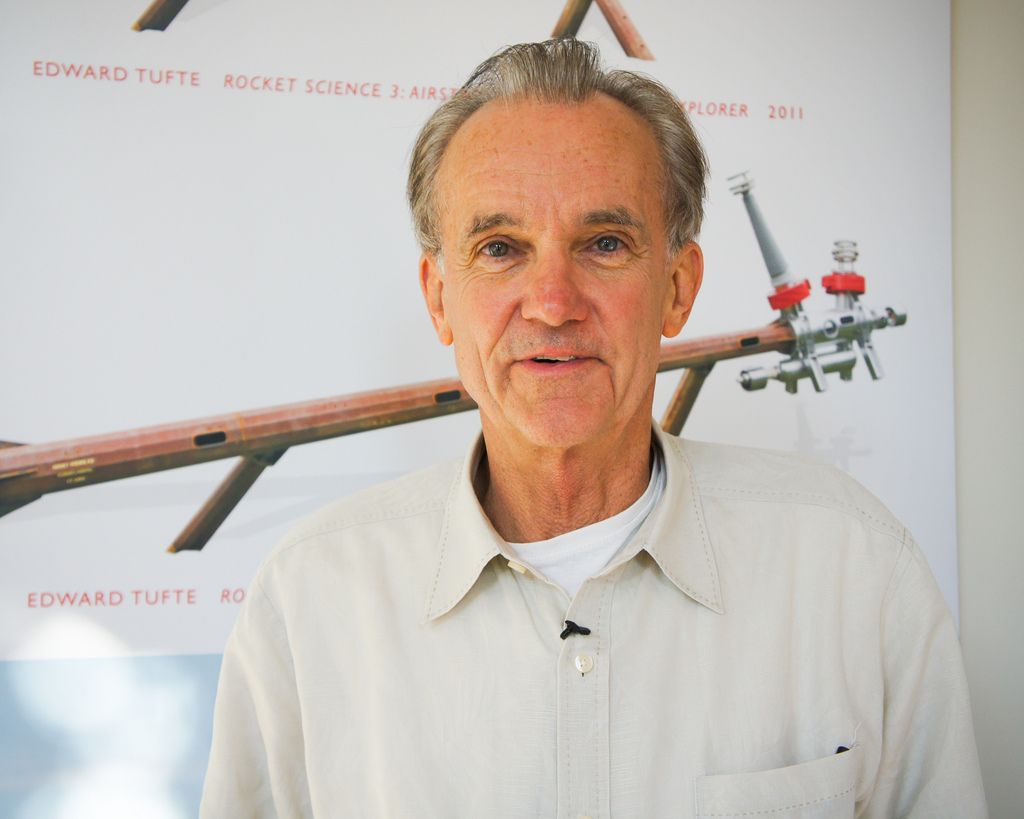
\includegraphics[width=0.95\textwidth]
				{images/edward-tufte.jpeg}
			\end{figure}
		\end{column}
		\begin{column}{0.5\textwidth}
			Tufte \cite[][page 92]{tufte2001} suggests to adhere to a
			basic design principle:

			\begin{quote}
				\textit{
					Show the data.

					\vspace{2em}

					The principle is the basis for a theory
					for a theory of data graphics.
				}
			\end{quote}
		\end{column}
	\end{columns}
\end{frame}

\begin{frame}{}{}
	\LARGE \centering Fine --- So What?!
\end{frame}

\begin{frame}{Maximize the Data-Ink Ratio!!}{}
	\begin{center}
		\begin{equation*}
			\text{Data-Ink ratio} = \frac{
				\text{data-ink}
			}
			{
				\text{total ink used to print the graphic design}
			}
		\end{equation*}
	\end{center}

	\vspace{2em}

	\textbf{Data-ink} is the non-erasable core of a graphic, the
	non-redundant ink arranged in response to variation in the numbers
	represented.
\end{frame}

\begin{frame}{Theee Versions of the Same Scatter Diagram}
	{Low data-ink ratio}
	\begin{figure}
		\begin{center}
			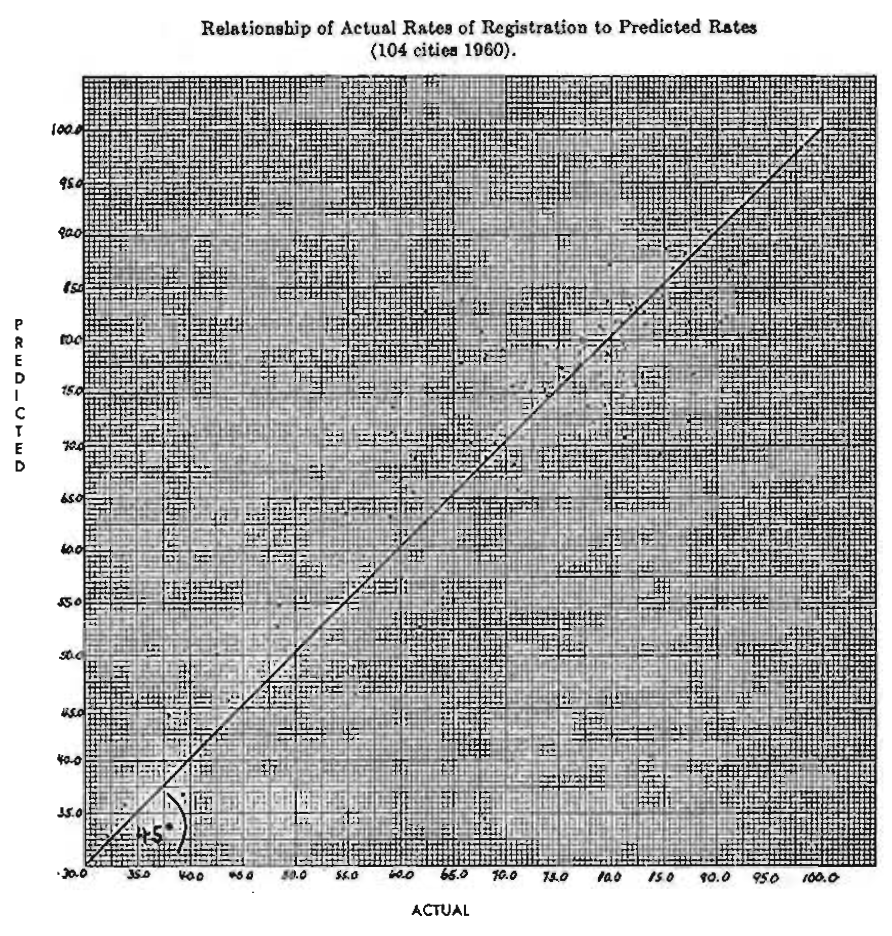
\includegraphics[width=0.55\textwidth]{images/low.png}
		\end{center}
	\end{figure}
\end{frame}

\begin{frame}{Theee Versions of the Same Scatter Diagram}
	{Substantial data-ink ratio}
	\begin{figure}
		\begin{center}
			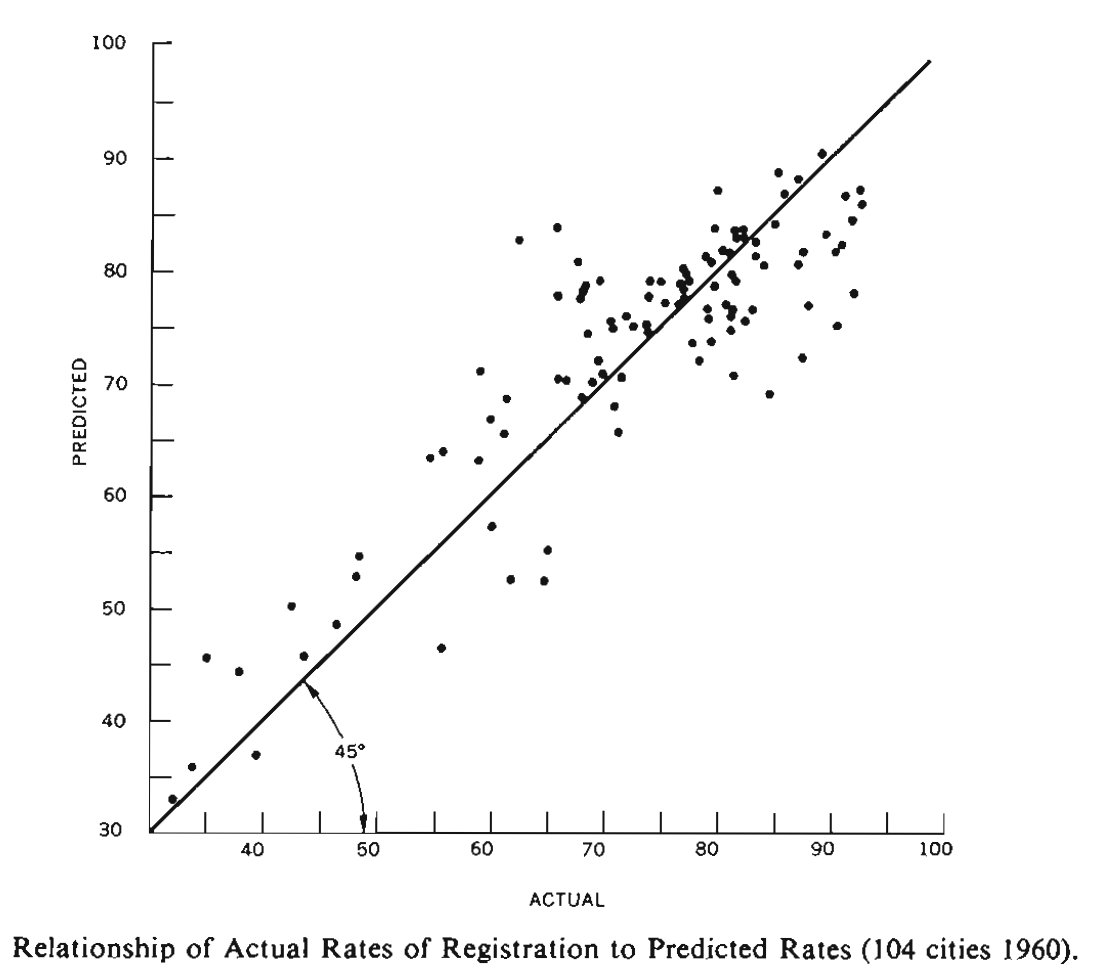
\includegraphics[width=0.6\textwidth]{images/high.png}
		\end{center}
	\end{figure}
\end{frame}

\begin{frame}{Theee Versions of the Same Scatter Diagram}
	{Null data-ink ratio}
	\begin{figure}
		\begin{center}
			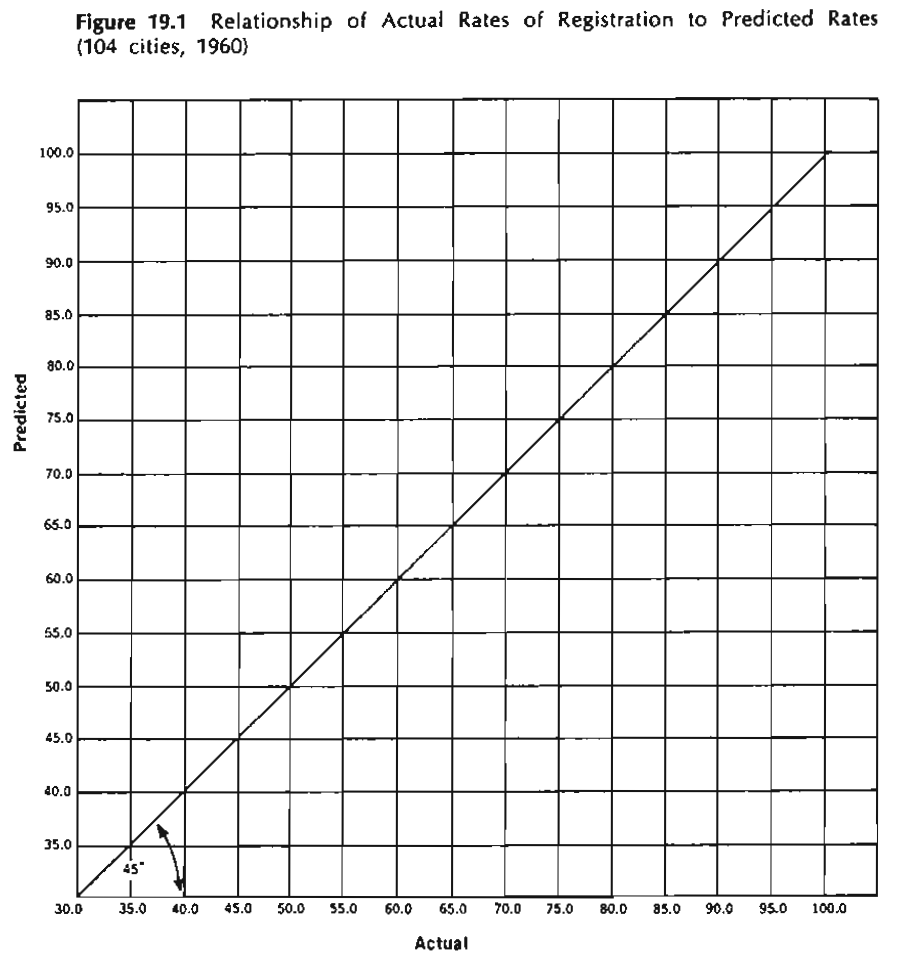
\includegraphics[width=0.5\textwidth]{images/null.png}
		\end{center}
	\end{figure}
\end{frame}

\begin{frame}{How to Improve the Data-Ink Ratio?}
	\begin{columns}[t]
		\begin{column}{0.5\textwidth}
			\begin{center}
				\textbf{Pre-chart execution:\\careful scoping}
			\end{center}
			\small
			\pause
			\begin{tcolorbox}[
					colback=blue!5!white,
					colframe=blue!60!black,
					title={
							\centering
							!! Maximize the data-ink ratio !!
						}]
				\raggedright Every bit of ink on a graphic requires a reason
				--- and the reason should be that the ink presents
				new information.
			\end{tcolorbox}

		\end{column}
		\pause
		\begin{column}{0.5\textwidth}
			\begin{center}
				\textbf{Post-chart execution:\\critical assessment}
			\end{center}
			\pause
			\small
			\begin{tcolorbox}[
					colback=blue!5!white,
					colframe=blue!60!green,
					title={
							\centering
							!! Erase the non data-ink !!
						}]
				\raggedright Non data-ink data clutters up the data, as is the case
				of a thick mesh of grid lines, or gratuitious
				decorations.
			\end{tcolorbox}

			\pause

			\begin{tcolorbox}[
					colback=blue!5!white,
					colframe=blue!60!green,
					title={
							\centering
							!! Erase redundant data-ink !!
						}]
				\raggedright Bilateral symmetry of data meausures also creates
				redundancy as in the box plot and the open bar.
			\end{tcolorbox}

		\end{column}
	\end{columns}
\end{frame}

% ========================== Chartjunk - not to do =========================

\section{Chartjunks --- How Not To Design a Chart}

\begin{frame}{Chartjunk? Give me a Break!!}{}
	\begin{quote}
		\textit
		``The interior decoration of graphics generates a lot of ink that not thell the
		viewer anything new. The purpose of decoration varies — to make the graphic
		appear more scientific and precise, to enliven the display, to give the designer
		an opportunity to exercise artistics skills. Regardless of its cause, it is all
		non data-data-ink or redundant data-ink, and it is often chartjunk.''
	\end{quote}

	\raggedleft --- Source is \cite[][page 107]{tufte2001}
\end{frame}

\begin{frame}
	{Moir\'e Effects}
	{...geometric shapes creating a sense of movement}
	\begin{figure}
		\begin{center}
			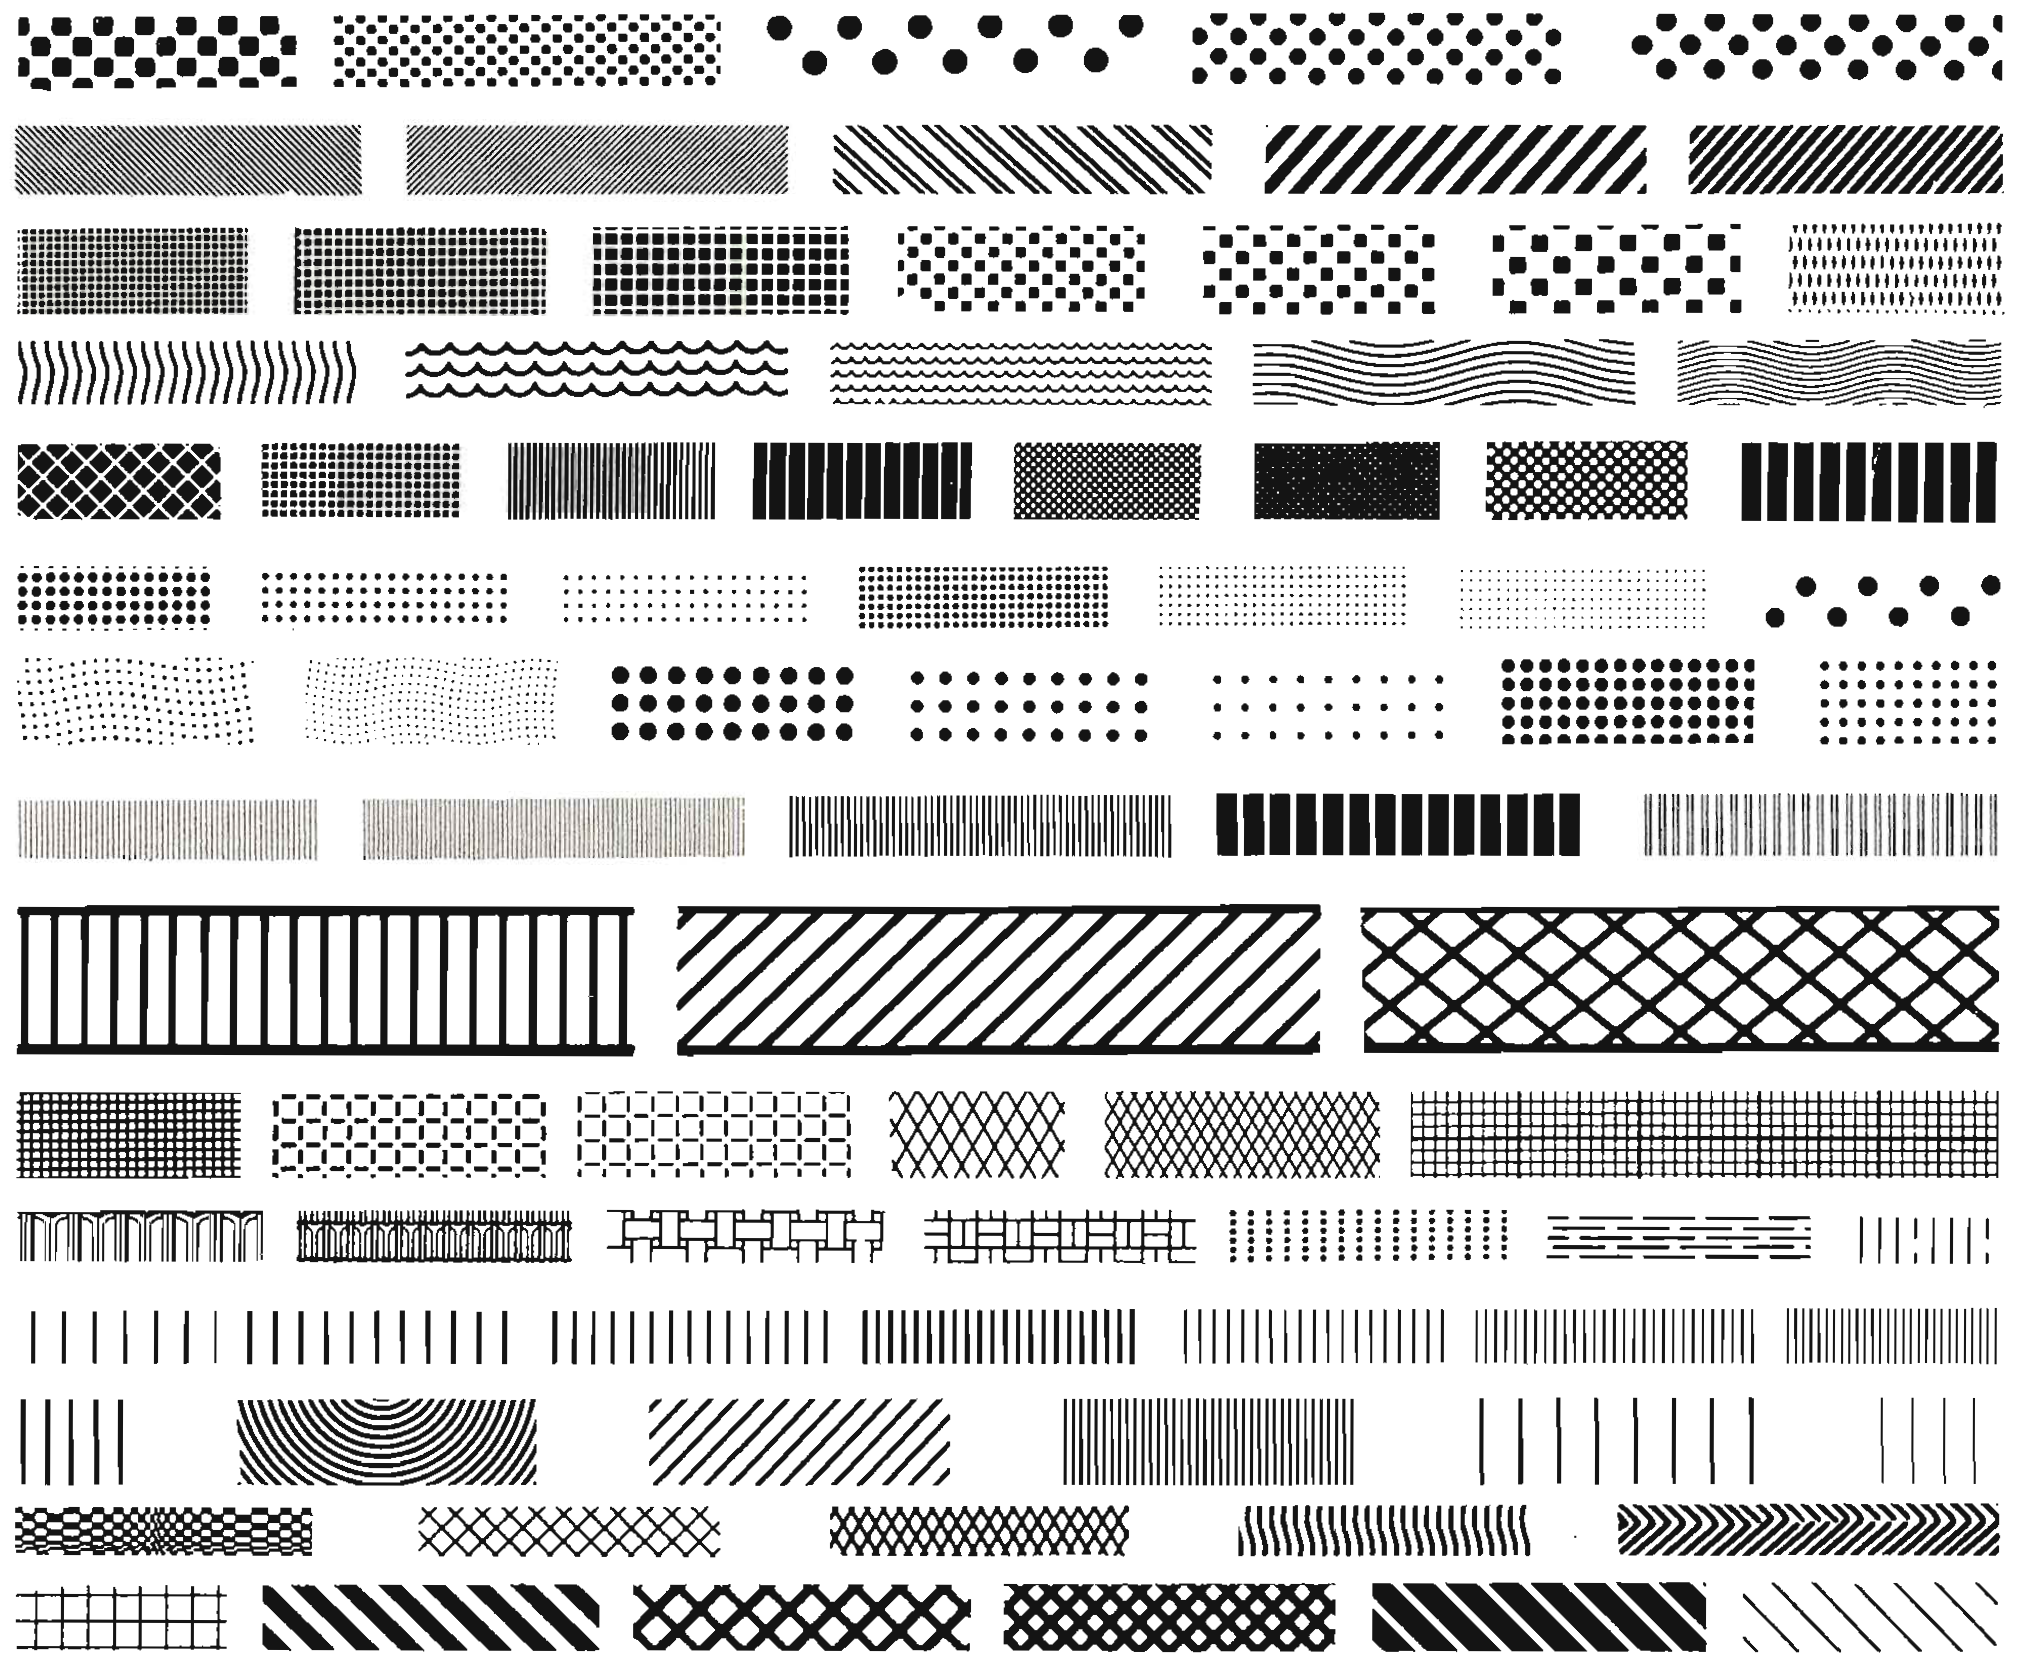
\includegraphics[width=0.7\textwidth]
			{images/moire_effects.png}
		\end{center}
	\end{figure}
\end{frame}

\begin{frame}
	{Get Rid of Moir\'e Effects}
	{Example 1 --- Source is ``Instituto de Expansao Commercial (1929)''}
	\centering
	\begin{figure}
		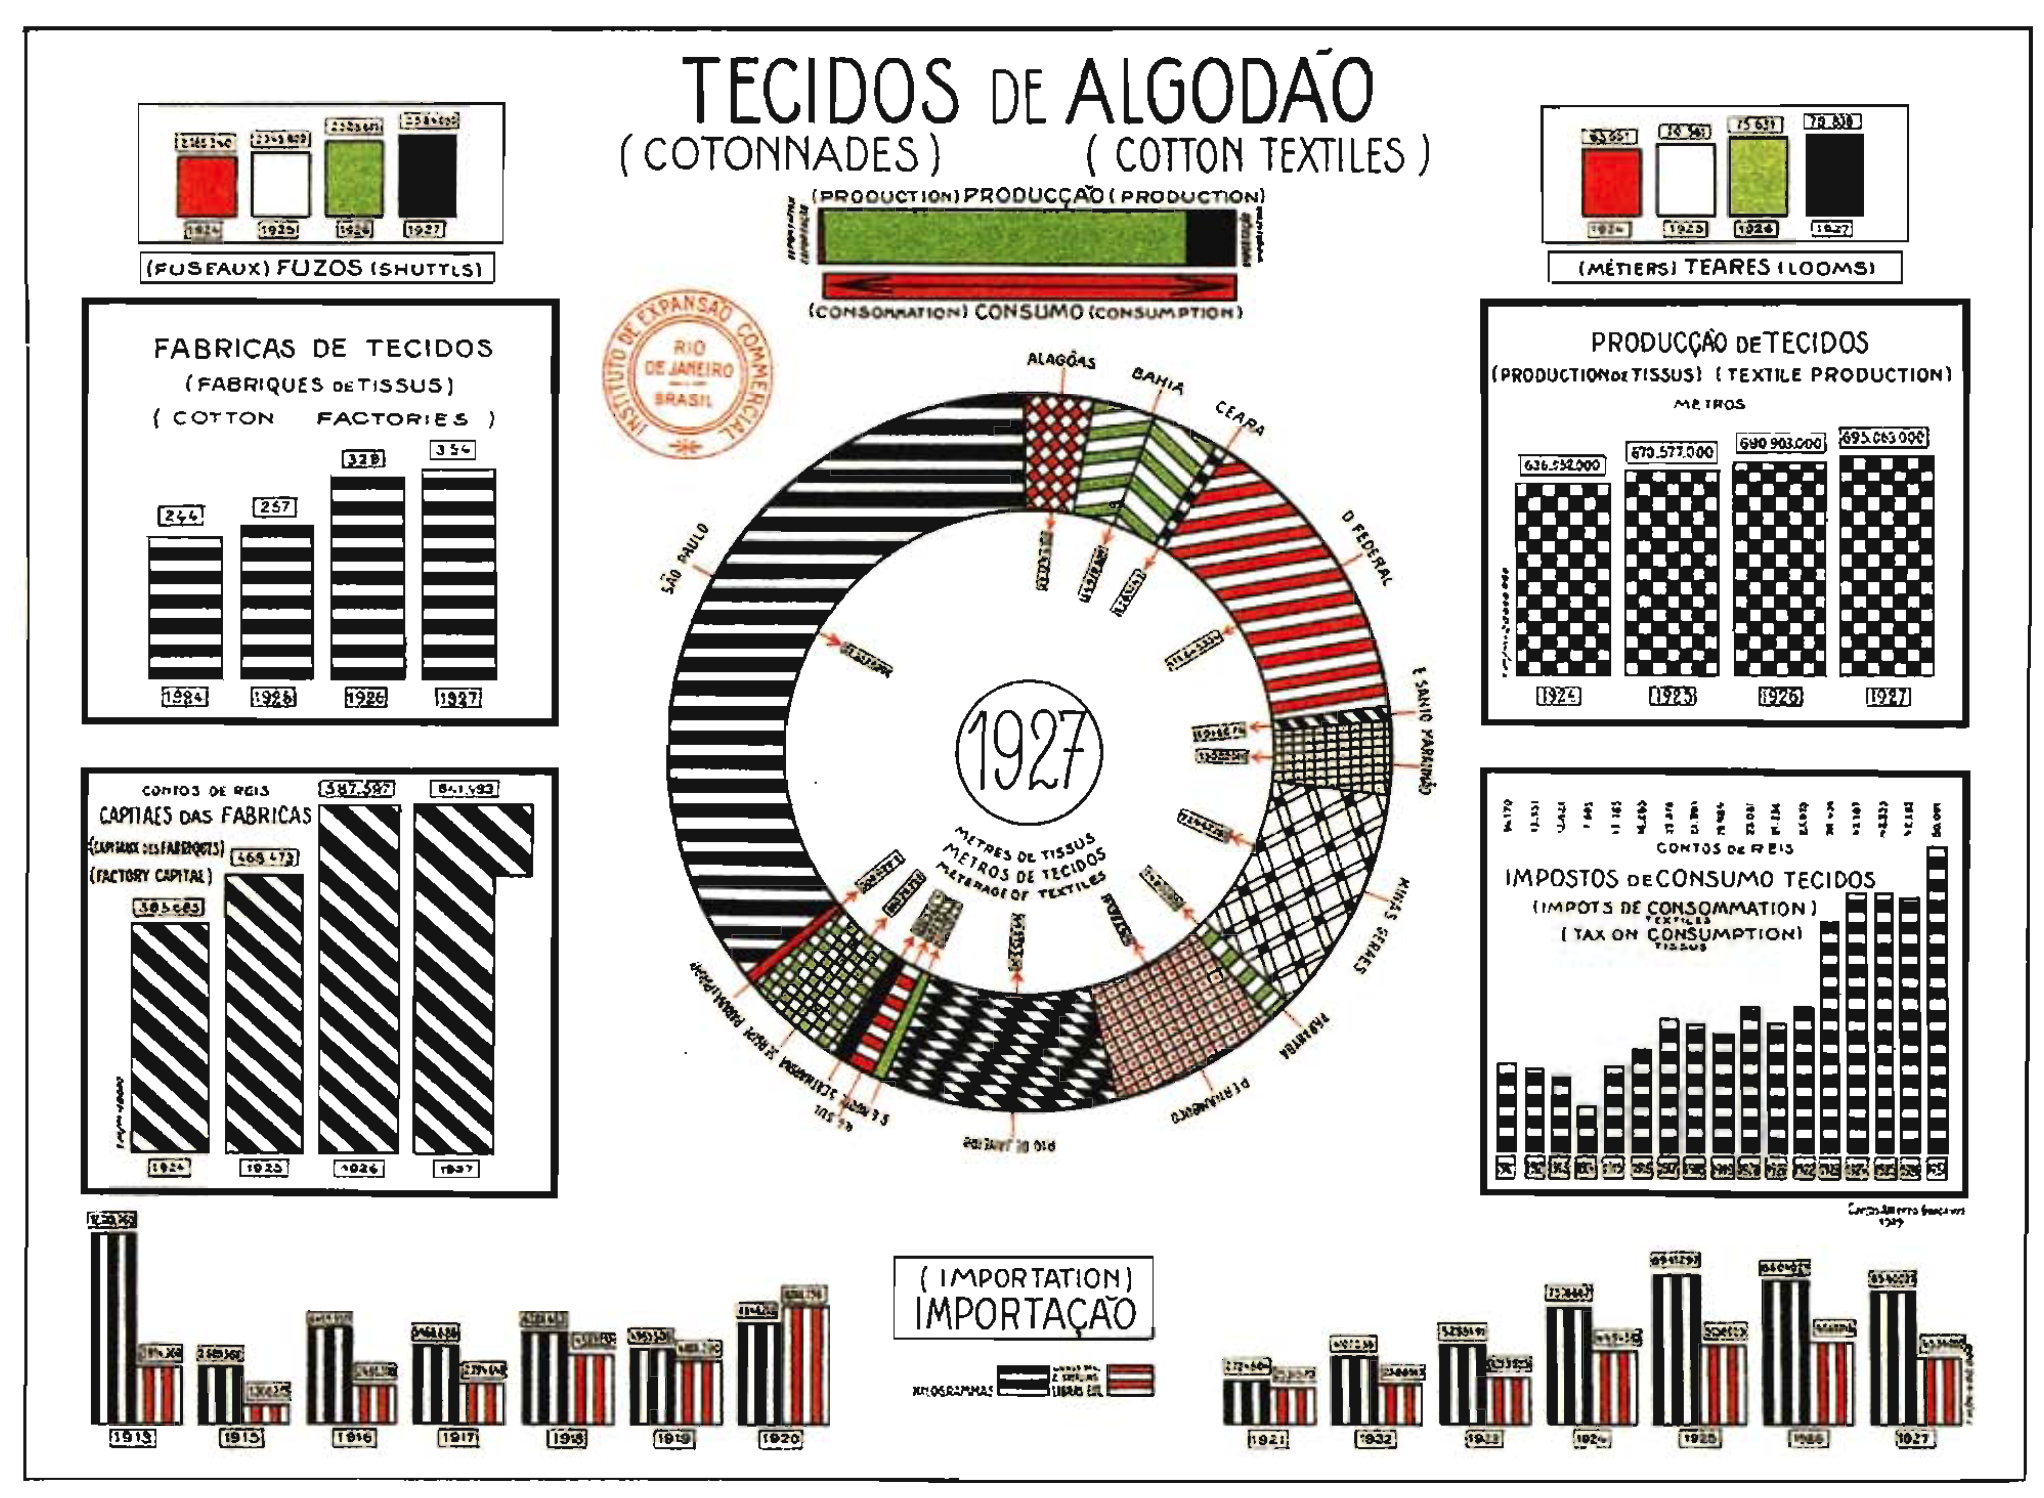
\includegraphics[width=0.7\textwidth]{images/moire_effect_1.png}
	\end{figure}
\end{frame}

\begin{frame}
	{Get Rid of Moir\'e Effects}
	{Example 2 --- Source is``Kouchoukos et al. (1994), New England Journal of Medicine''}
	\centering
	\begin{figure}
		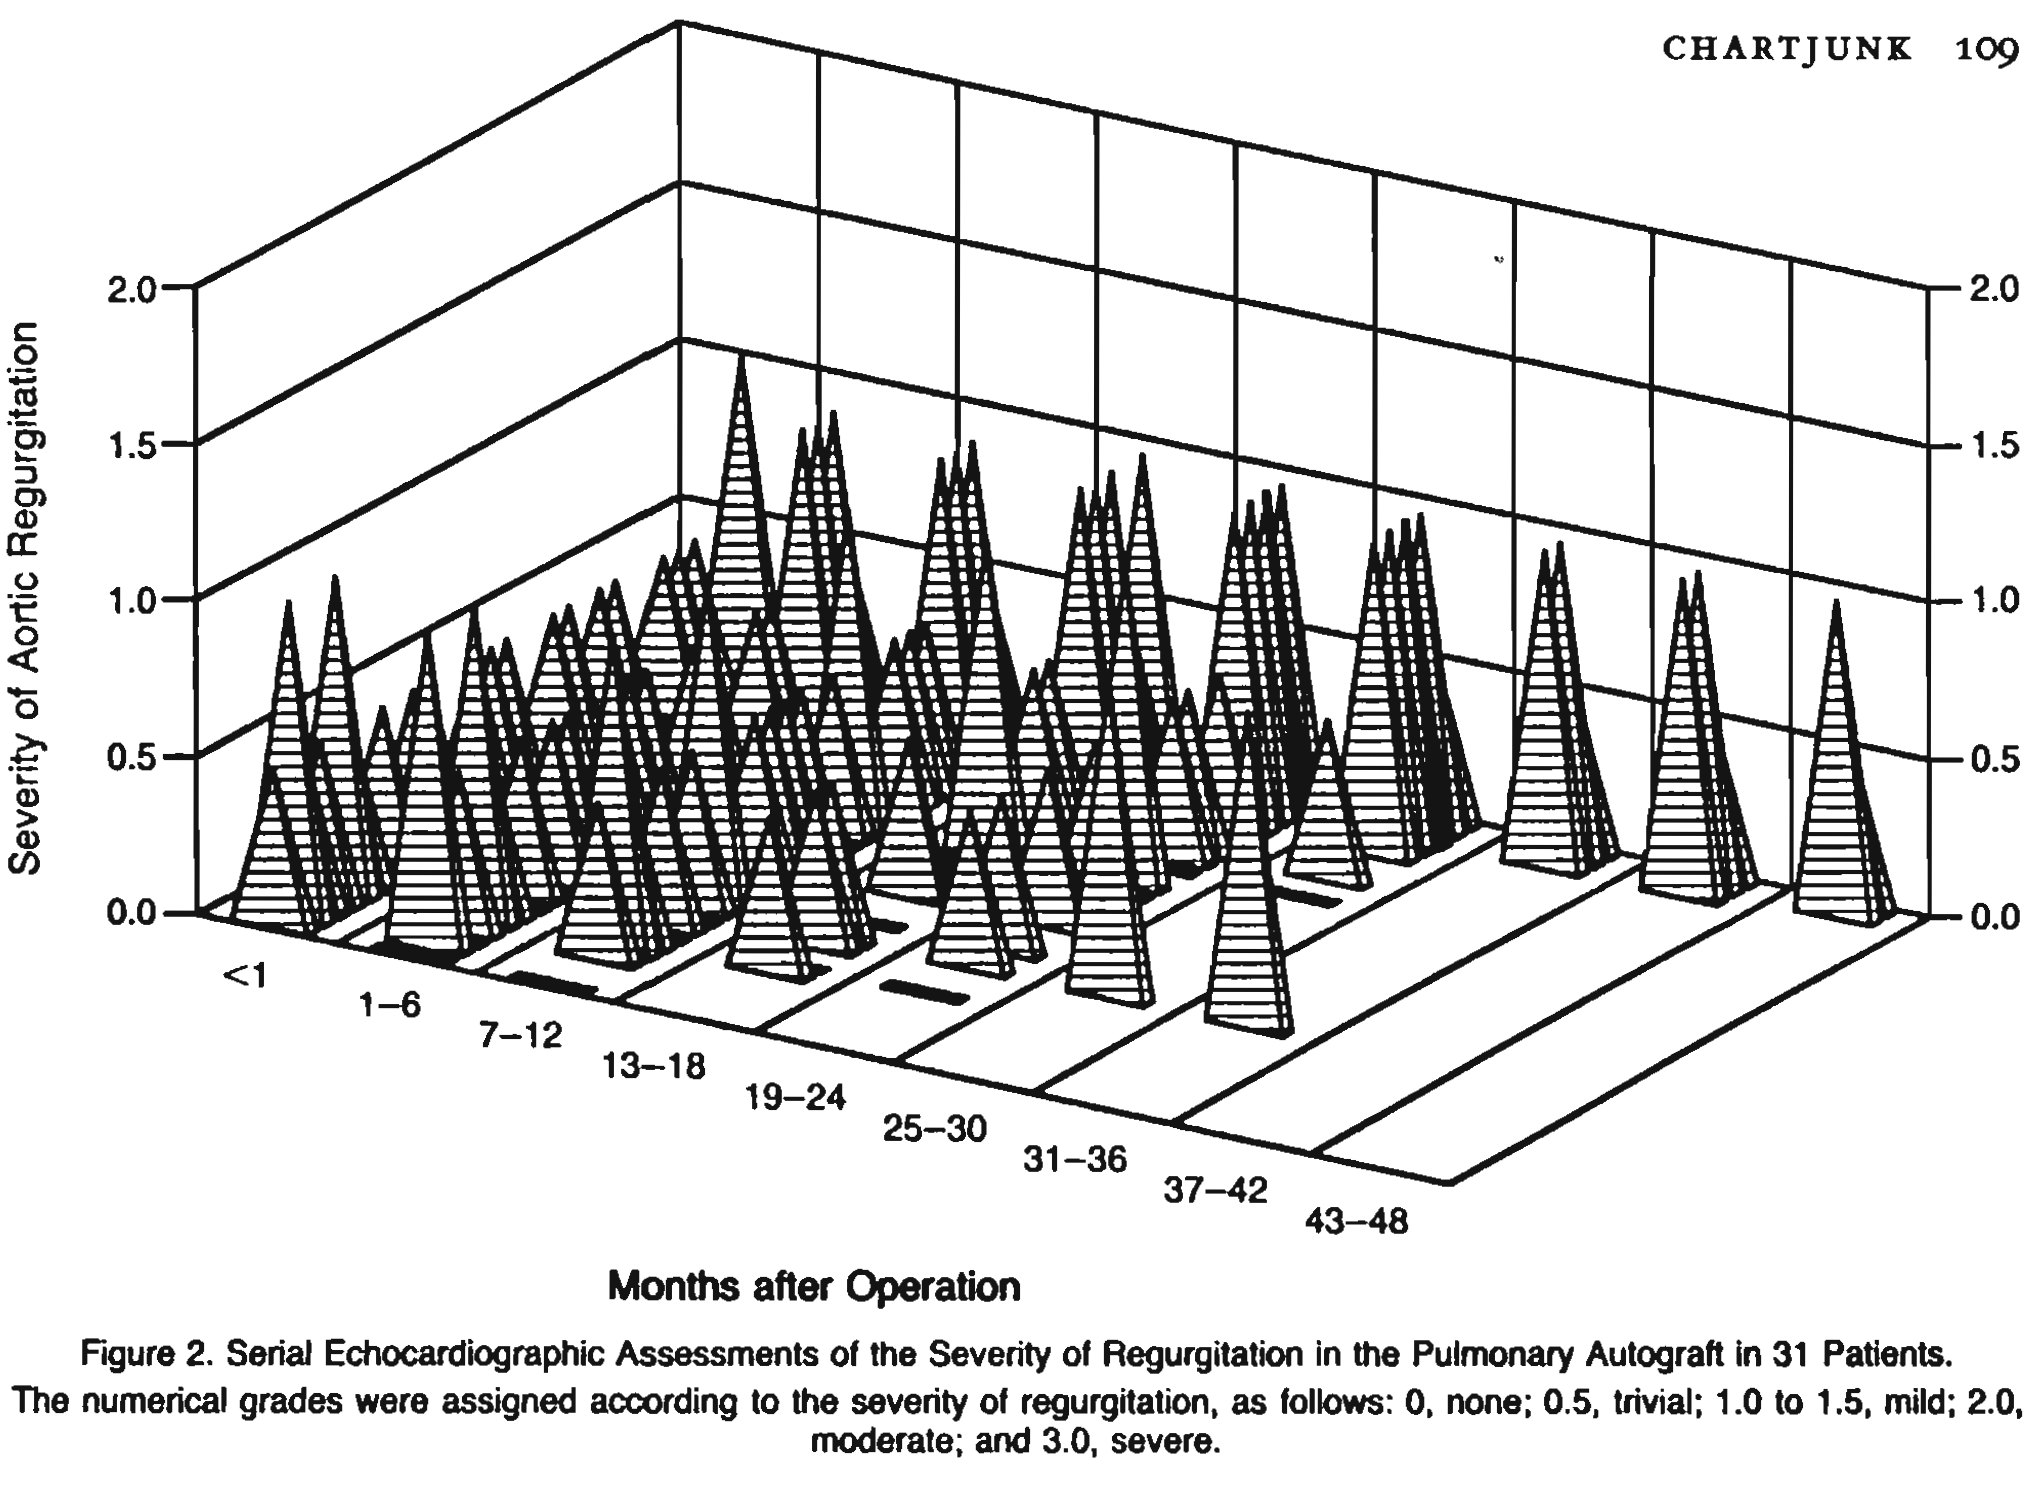
\includegraphics[width=0.7\textwidth]{images/moire_effect_2.png}
	\end{figure}
\end{frame}

\begin{frame}
	{Get Rid of Moir\'e Effects}
	{Example 3 --- Source is ``JASA style sheet (1976), Journal of the American Statistical Association''}
	\centering
	\begin{figure}
		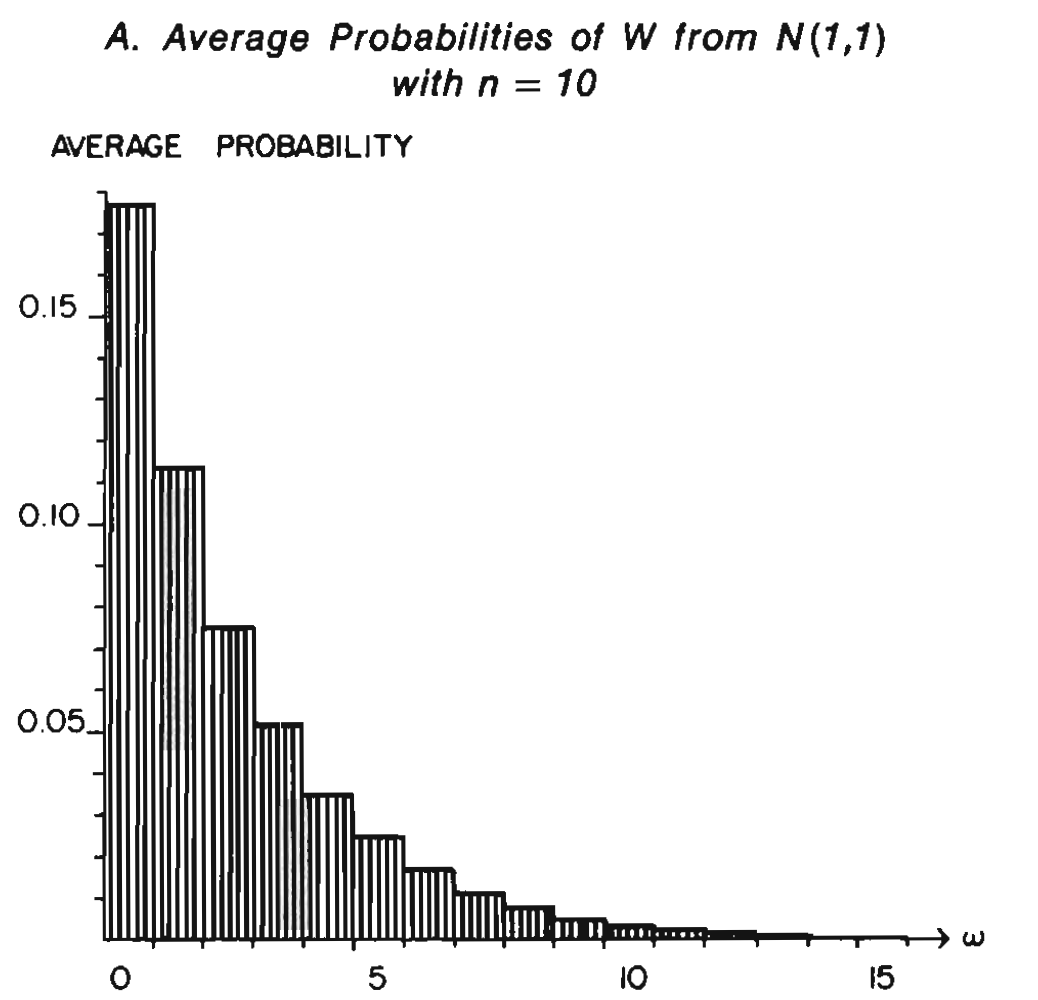
\includegraphics[width=0.6\textwidth]{images/moire_effect_3.png}
	\end{figure}
\end{frame}

\begin{frame}
	{Use Grids Conscientiously}
	{Example --- Source is ``Institut National de la Statistique et des
		\'Etudes \'Economiques''}
	\centering
	\begin{figure}
		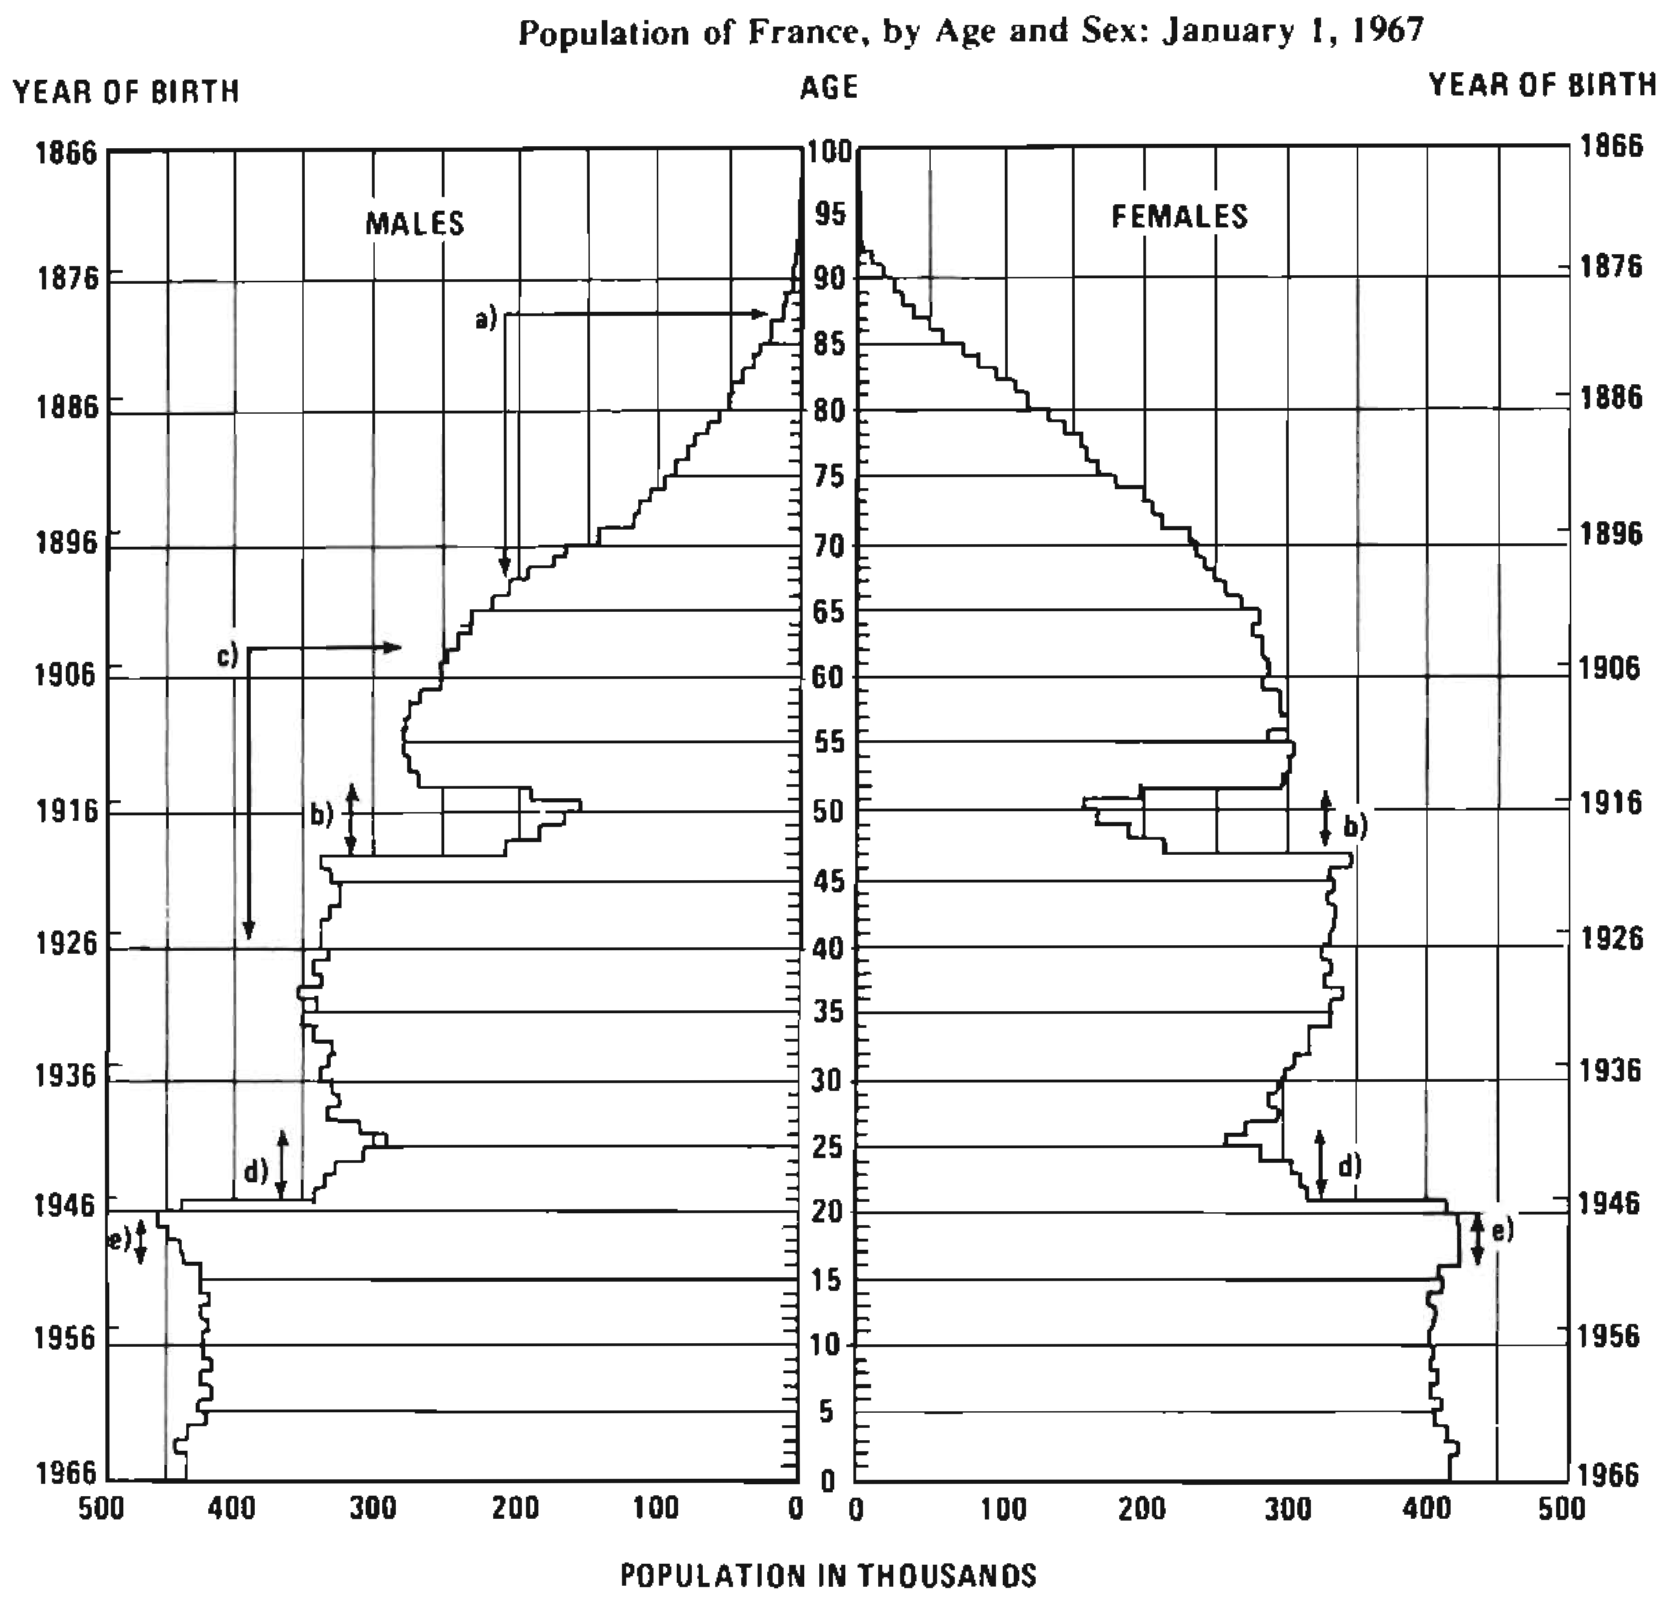
\includegraphics[width=0.6\textwidth]{images/grid_1.png}
	\end{figure}
\end{frame}

\begin{frame}
	{Use Grids Conscientiously}
	{Redesigning the previous example}
	\centering
	\begin{figure}
		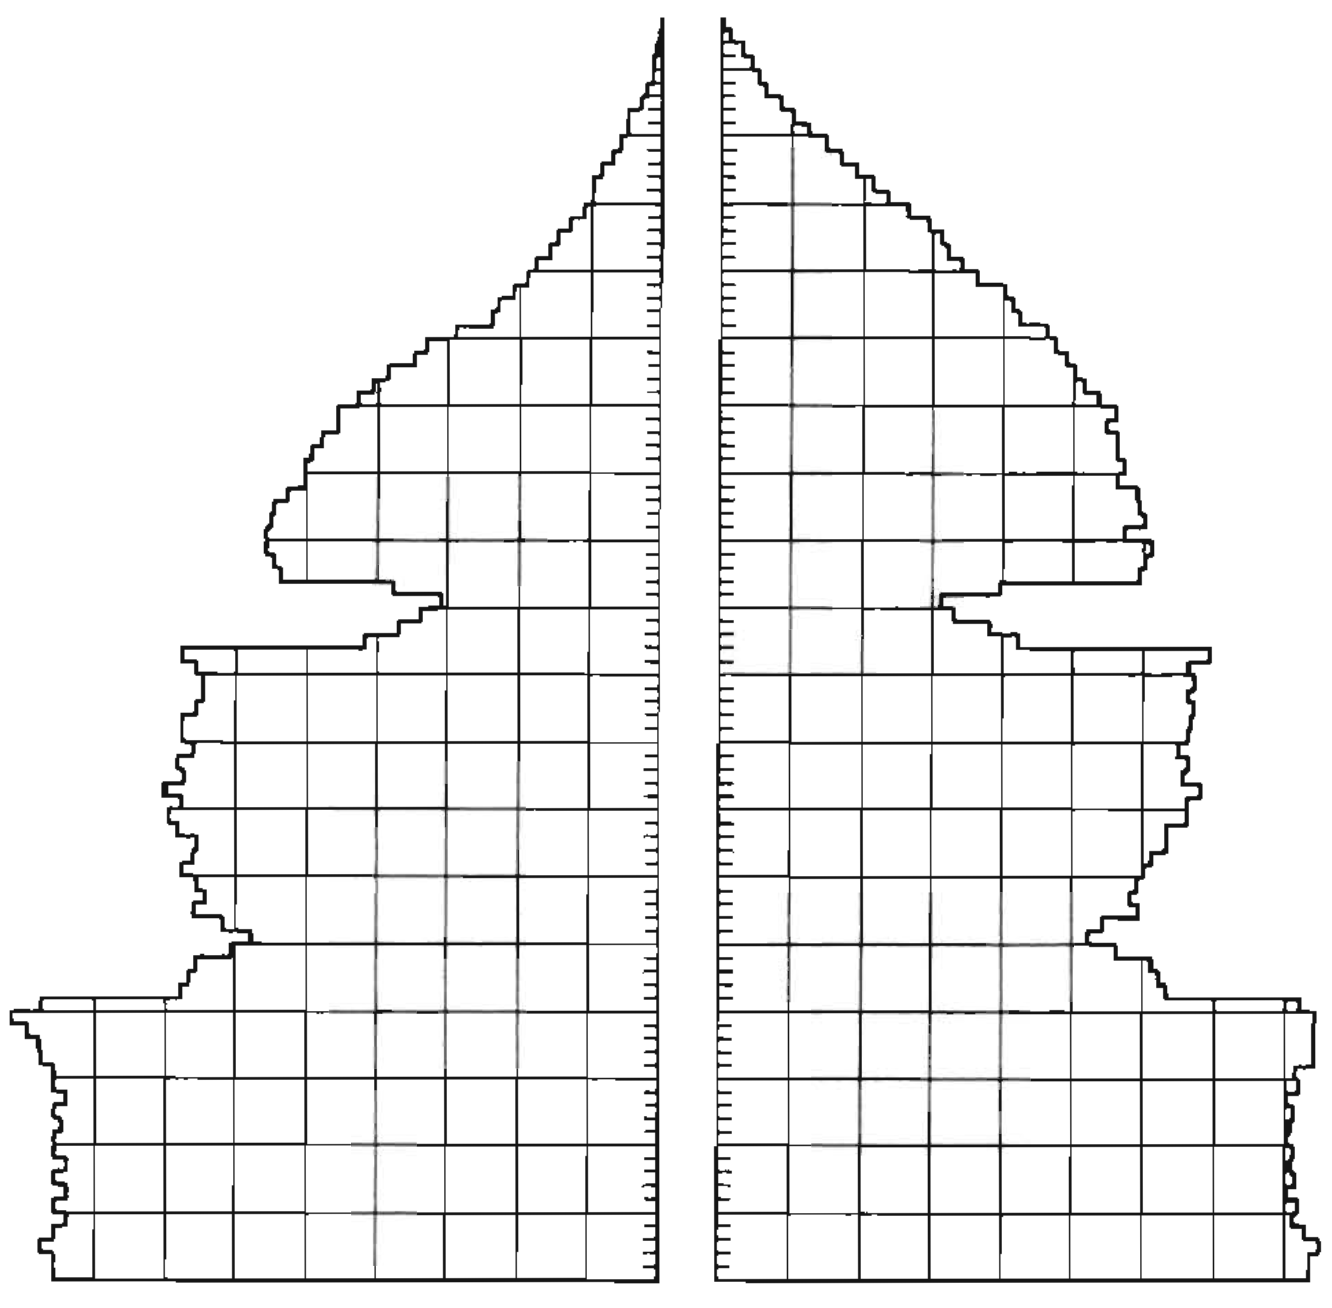
\includegraphics[width=0.6\textwidth]{images/grid_2.png}
	\end{figure}
\end{frame}

\begin{frame}{Have You Creted a `Duck Chart'?}{\textit{Big Duck}, Flanders,
		New York, photograph by Edward Tufte, July 2000.}
	\begin{figure}
		\begin{center}
			\includegraphics[width=0.7\textwidth]{images/big_duck.png}
		\end{center}
	\end{figure}
\end{frame}

\begin{frame}{An Example of `Duck Chart'}{Source is \cite[][page 118]{tufte2001}}
	\begin{figure}
		\begin{center}
			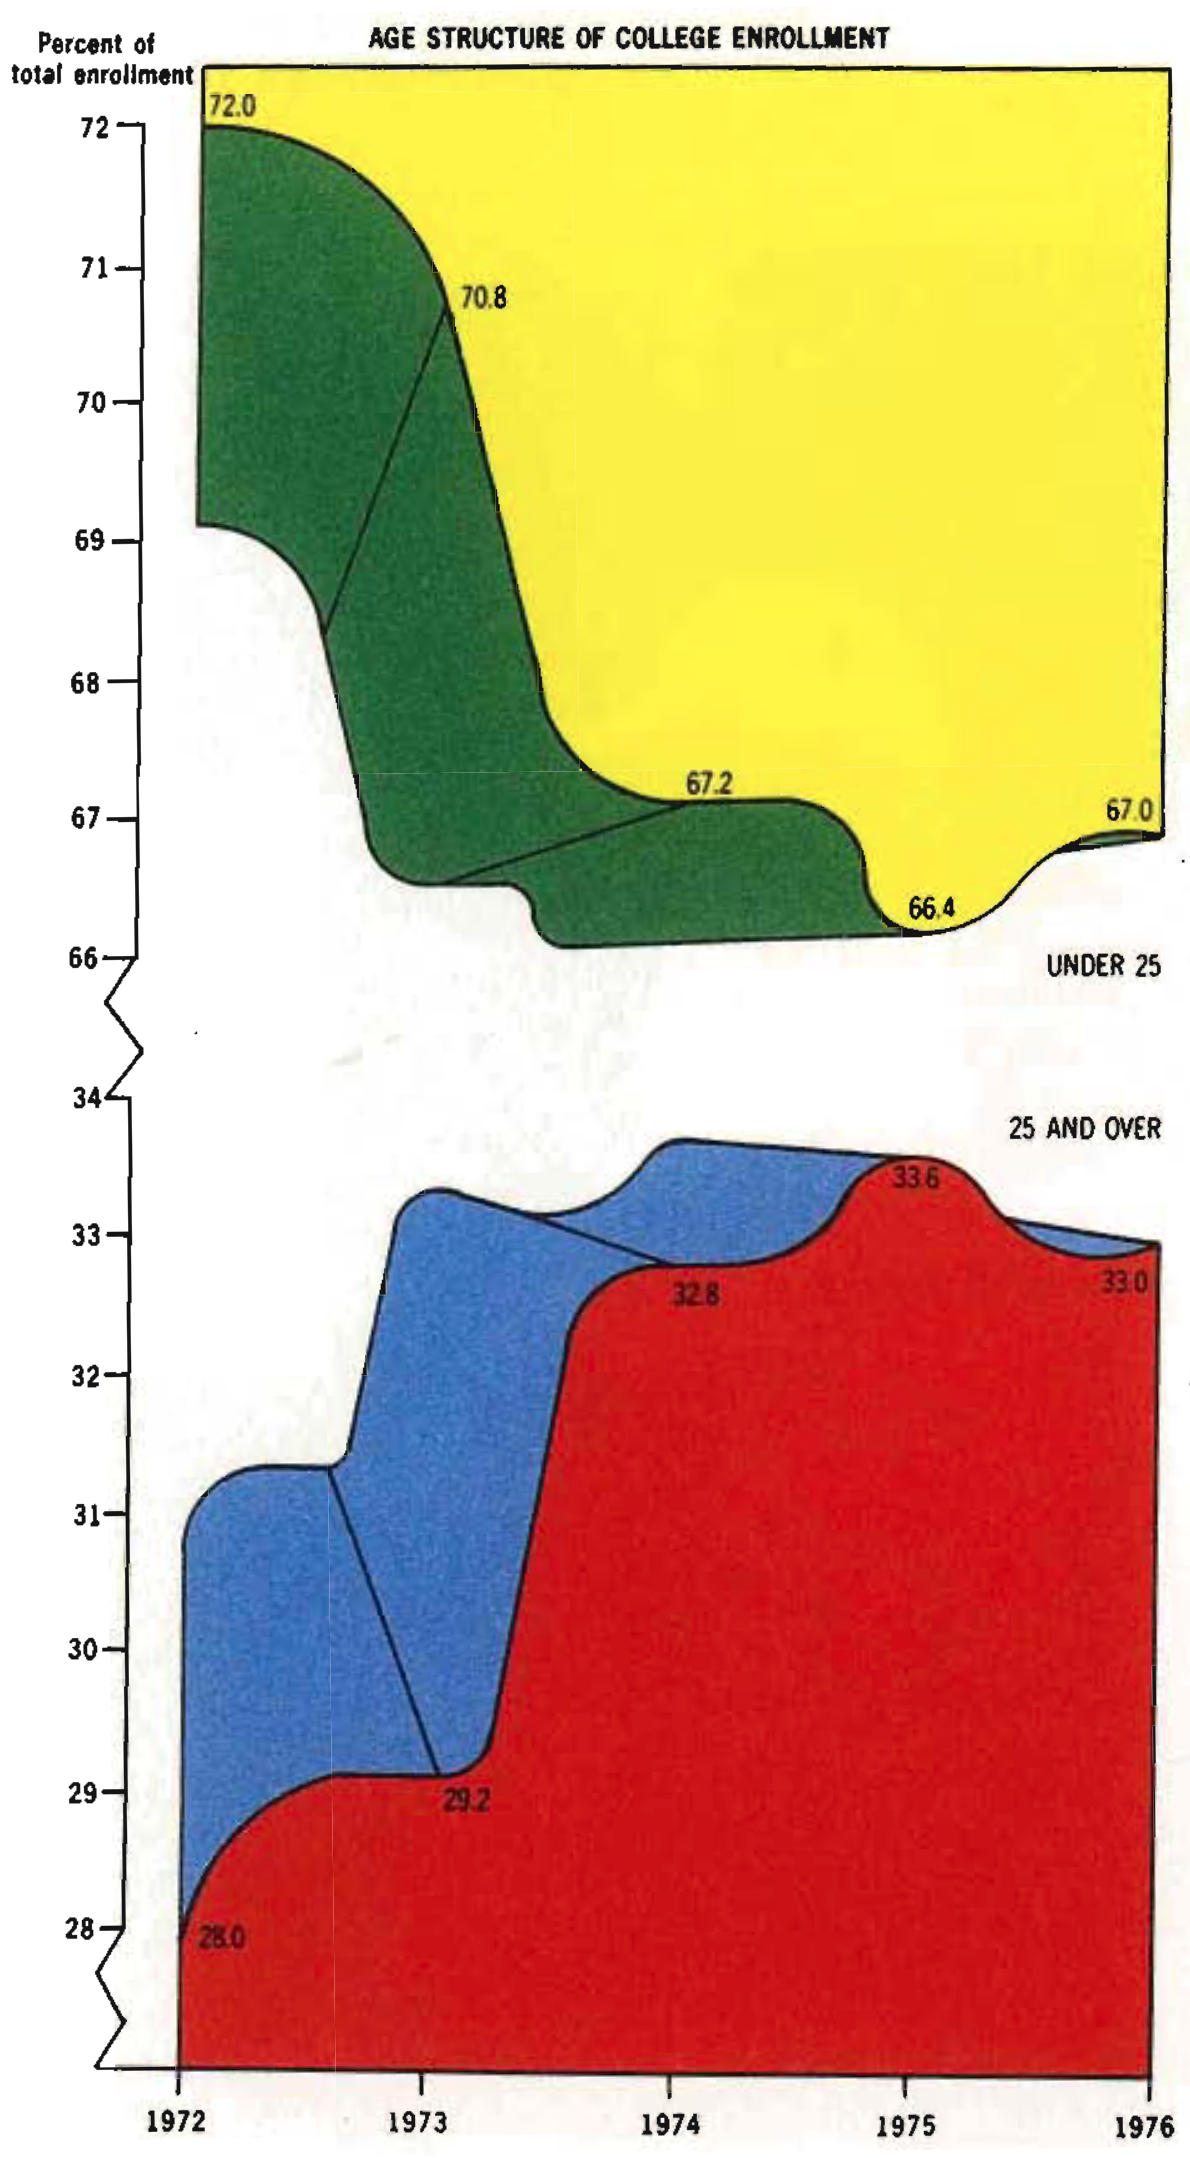
\includegraphics[width=0.5\textwidth]{images/a_duck_chart.png}
		\end{center}
	\end{figure}
\end{frame}

%% =========================== Redesigning stat charts =====================
\section{Redesigning Statistical Charts}

\begin{frame}{John Tukey's Box Plot}{}
	\begin{figure}
		\begin{center}
			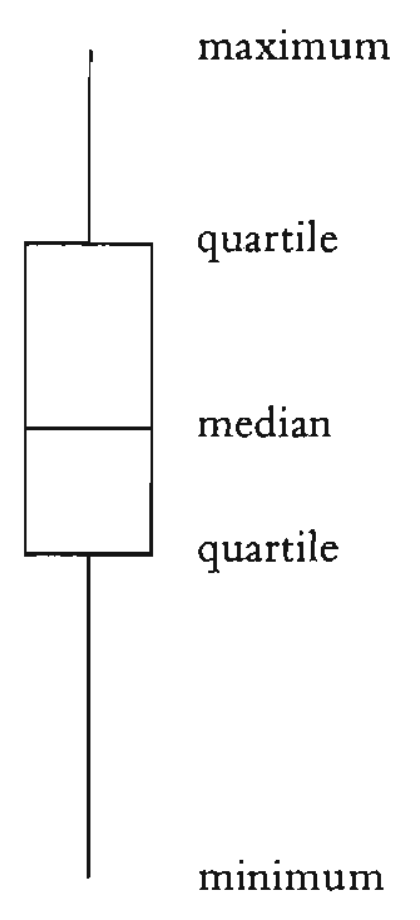
\includegraphics[width=0.25\textwidth]{images/boxplot.png}
		\end{center}
	\end{figure}
\end{frame}

\begin{frame}{A Box Plot with a Limited Data-Ink Ratio}{}
	\begin{figure}
		\begin{center}
			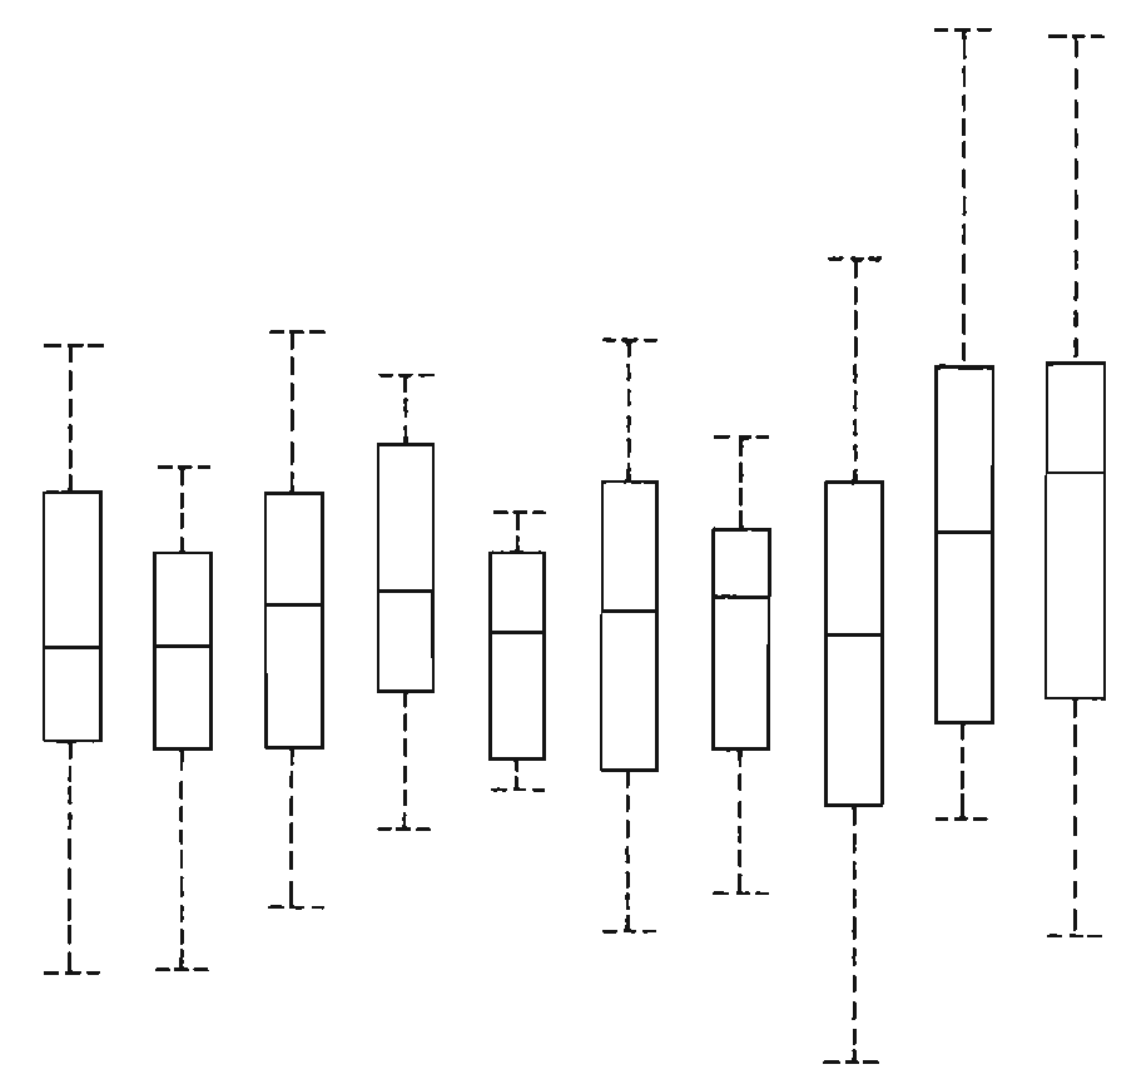
\includegraphics[width=0.6\textwidth]{images/trad_boxplot.png}
		\end{center}
	\end{figure}
\end{frame}

\begin{frame}{Tufte-Alike Box Plot}{}
	\begin{figure}
		\begin{center}
			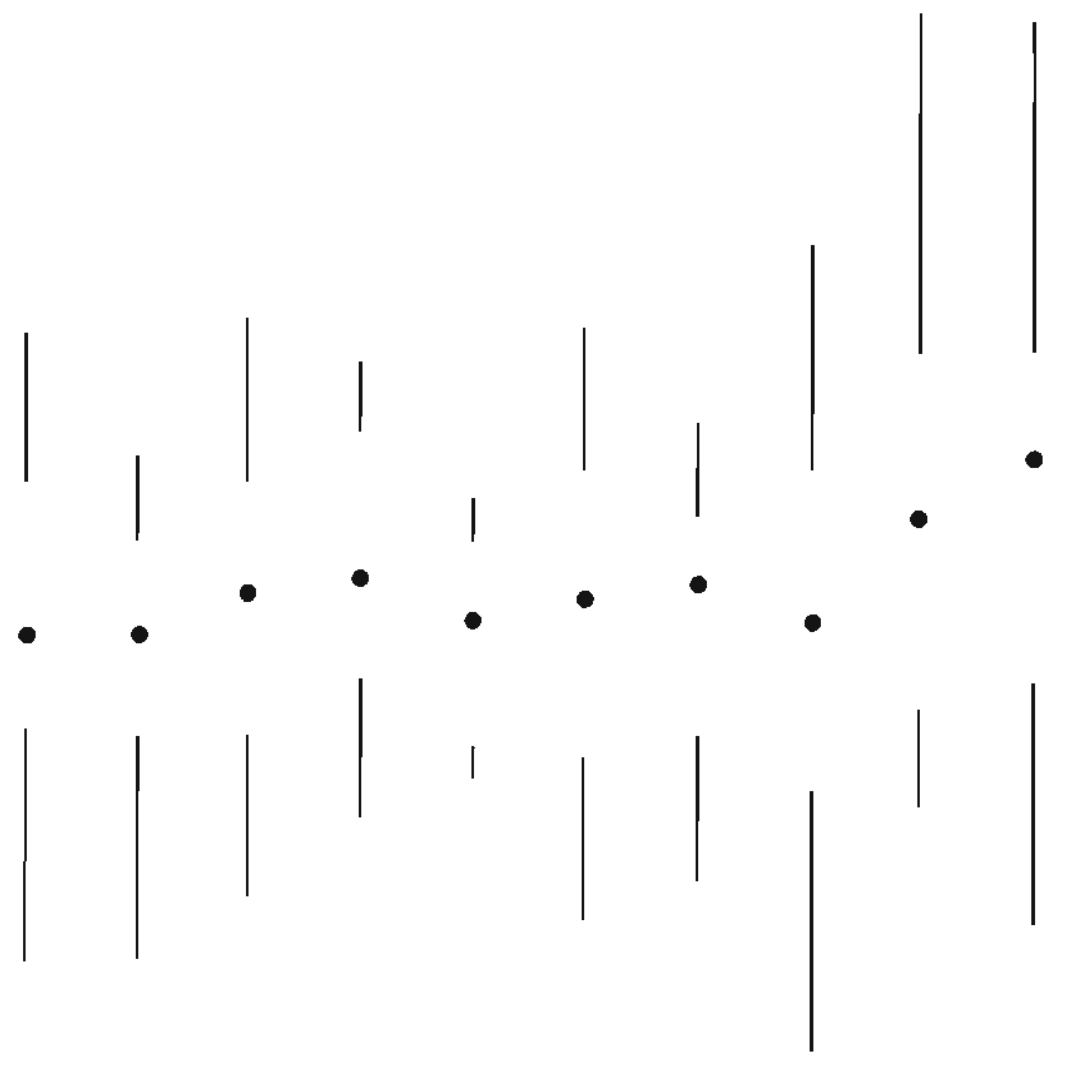
\includegraphics[width=0.6\textwidth]{images/tufte_boxplot.png}
		\end{center}
	\end{figure}

\end{frame}

\begin{frame}{A Bar Chart with a Limited Data-Ink Ratio}{}
	\begin{figure}
		\begin{center}
			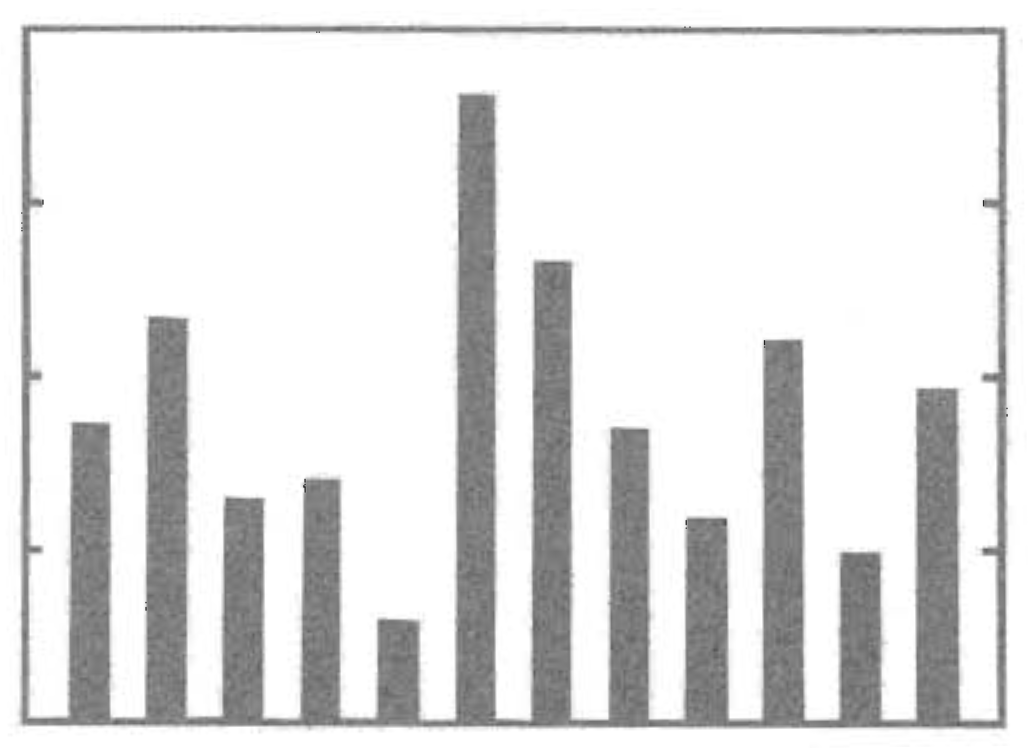
\includegraphics[width=0.75\textwidth]{images/trad_barchart.png}
		\end{center}
	\end{figure}

\end{frame}

\begin{frame}{Tufte-Alike Bar Chart}{}
	\begin{figure}
		\begin{center}
			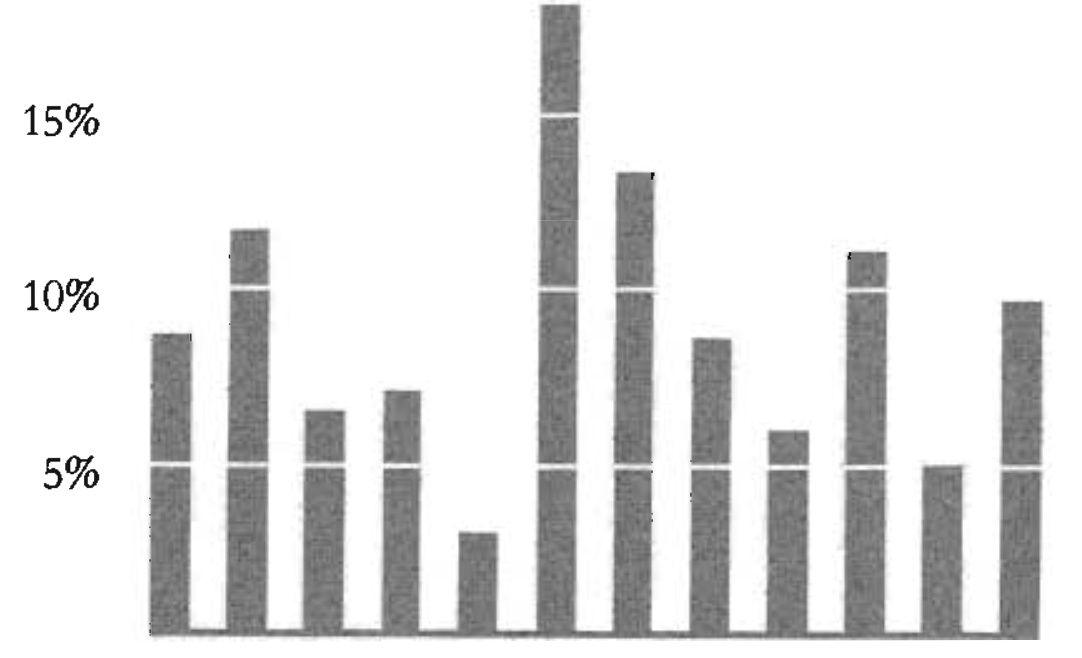
\includegraphics[width=0.8\textwidth]{images/tufte_barchart.png}
		\end{center}
	\end{figure}

\end{frame}

\begin{frame}{A Bare-Bone Scatter Diagram}{}
	\begin{figure}
		\begin{center}
			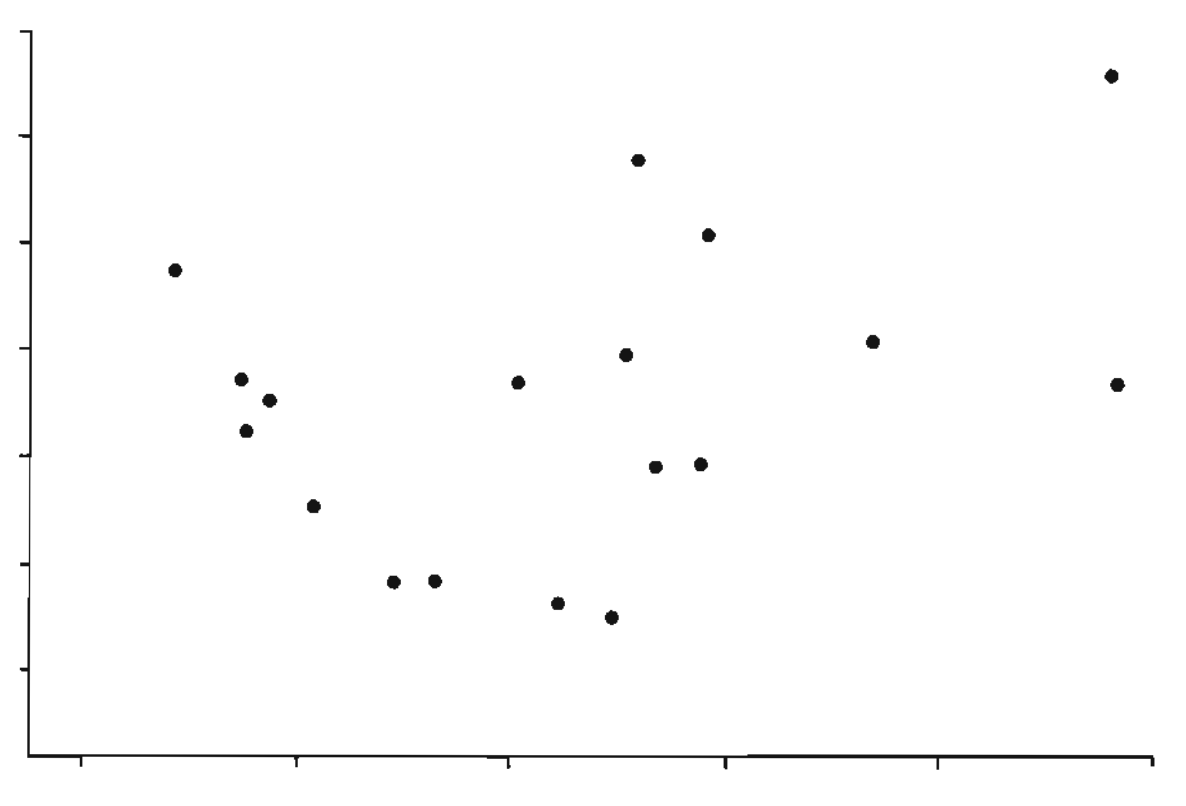
\includegraphics[width=0.8\textwidth]{images/trad_scatter.png}
		\end{center}
	\end{figure}

\end{frame}

\begin{frame}{Tufte-Alike Scatter Diagram}{}
	\begin{figure}
		\begin{center}
			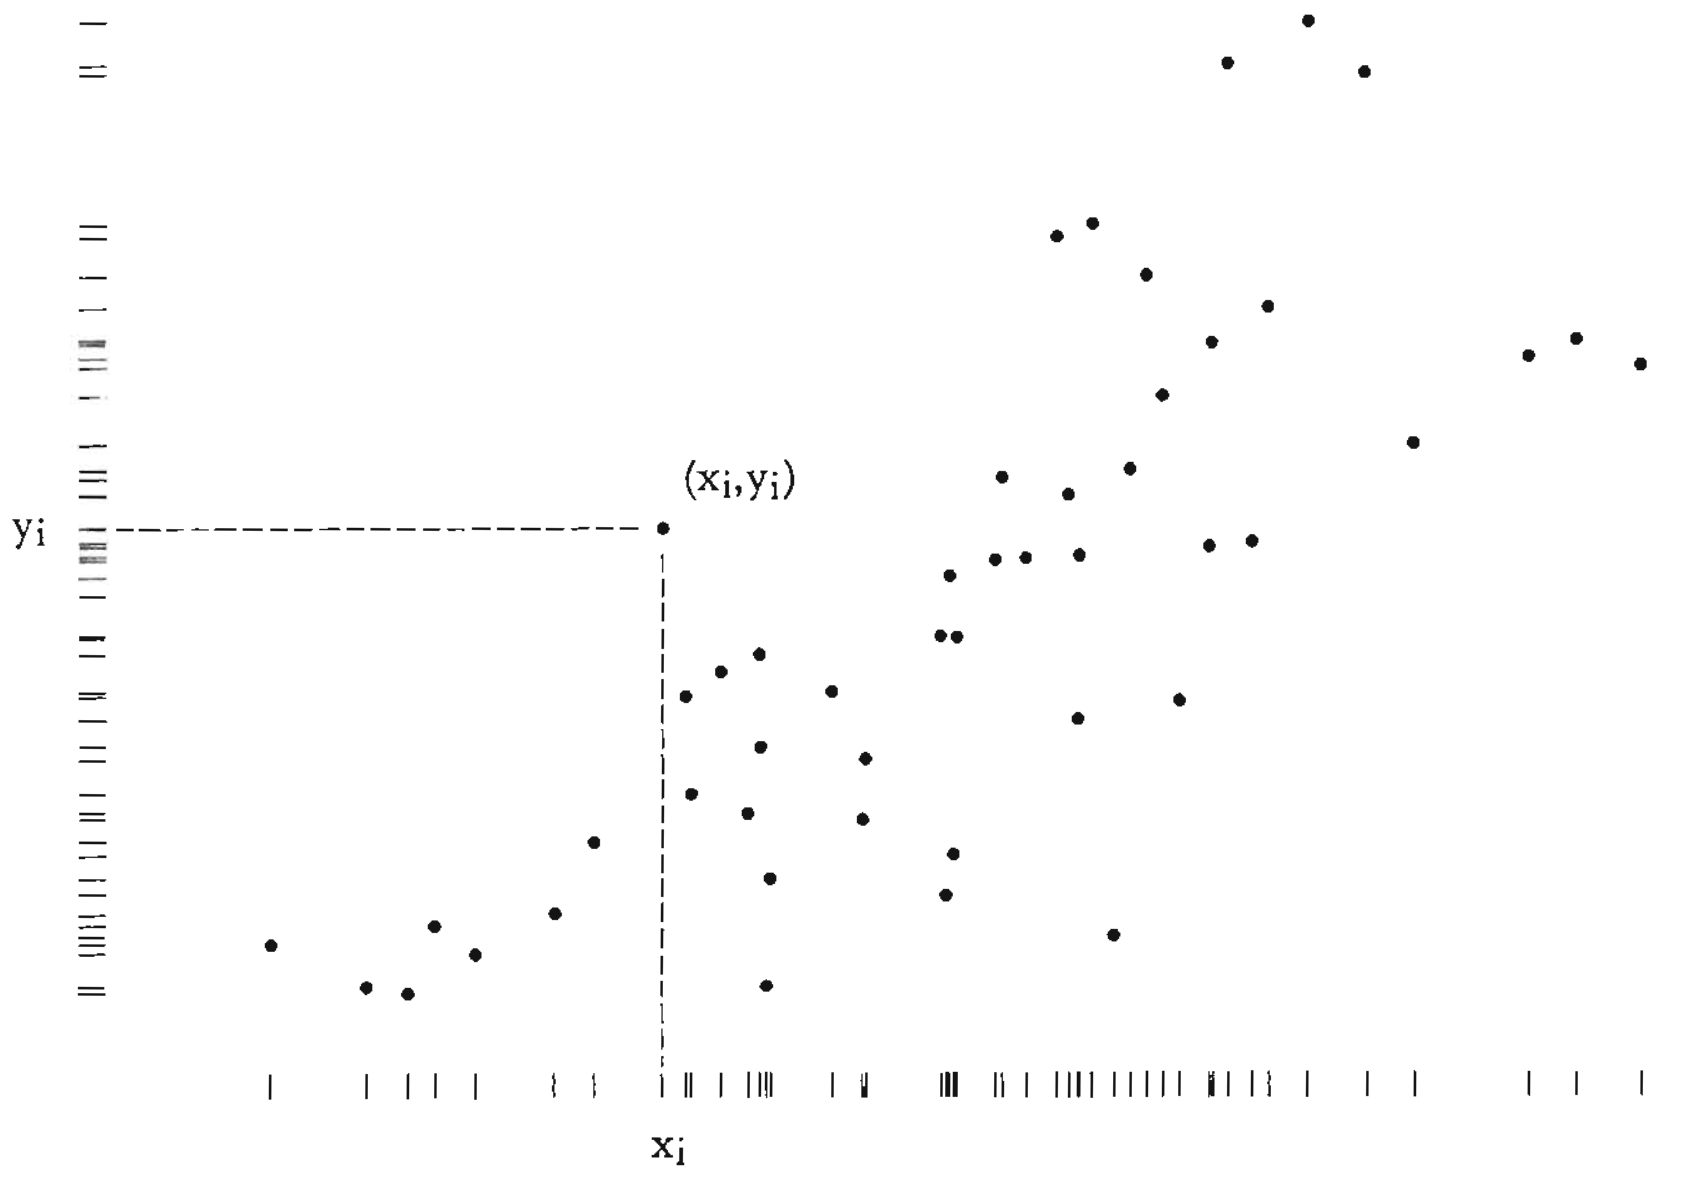
\includegraphics[width=0.85\textwidth]{images/tufte_scatter.png}
		\end{center}
	\end{figure}

\end{frame}

\begin{frame}{Tufte-Alike Scatter Diagram}{}
	\begin{figure}
		\begin{center}
			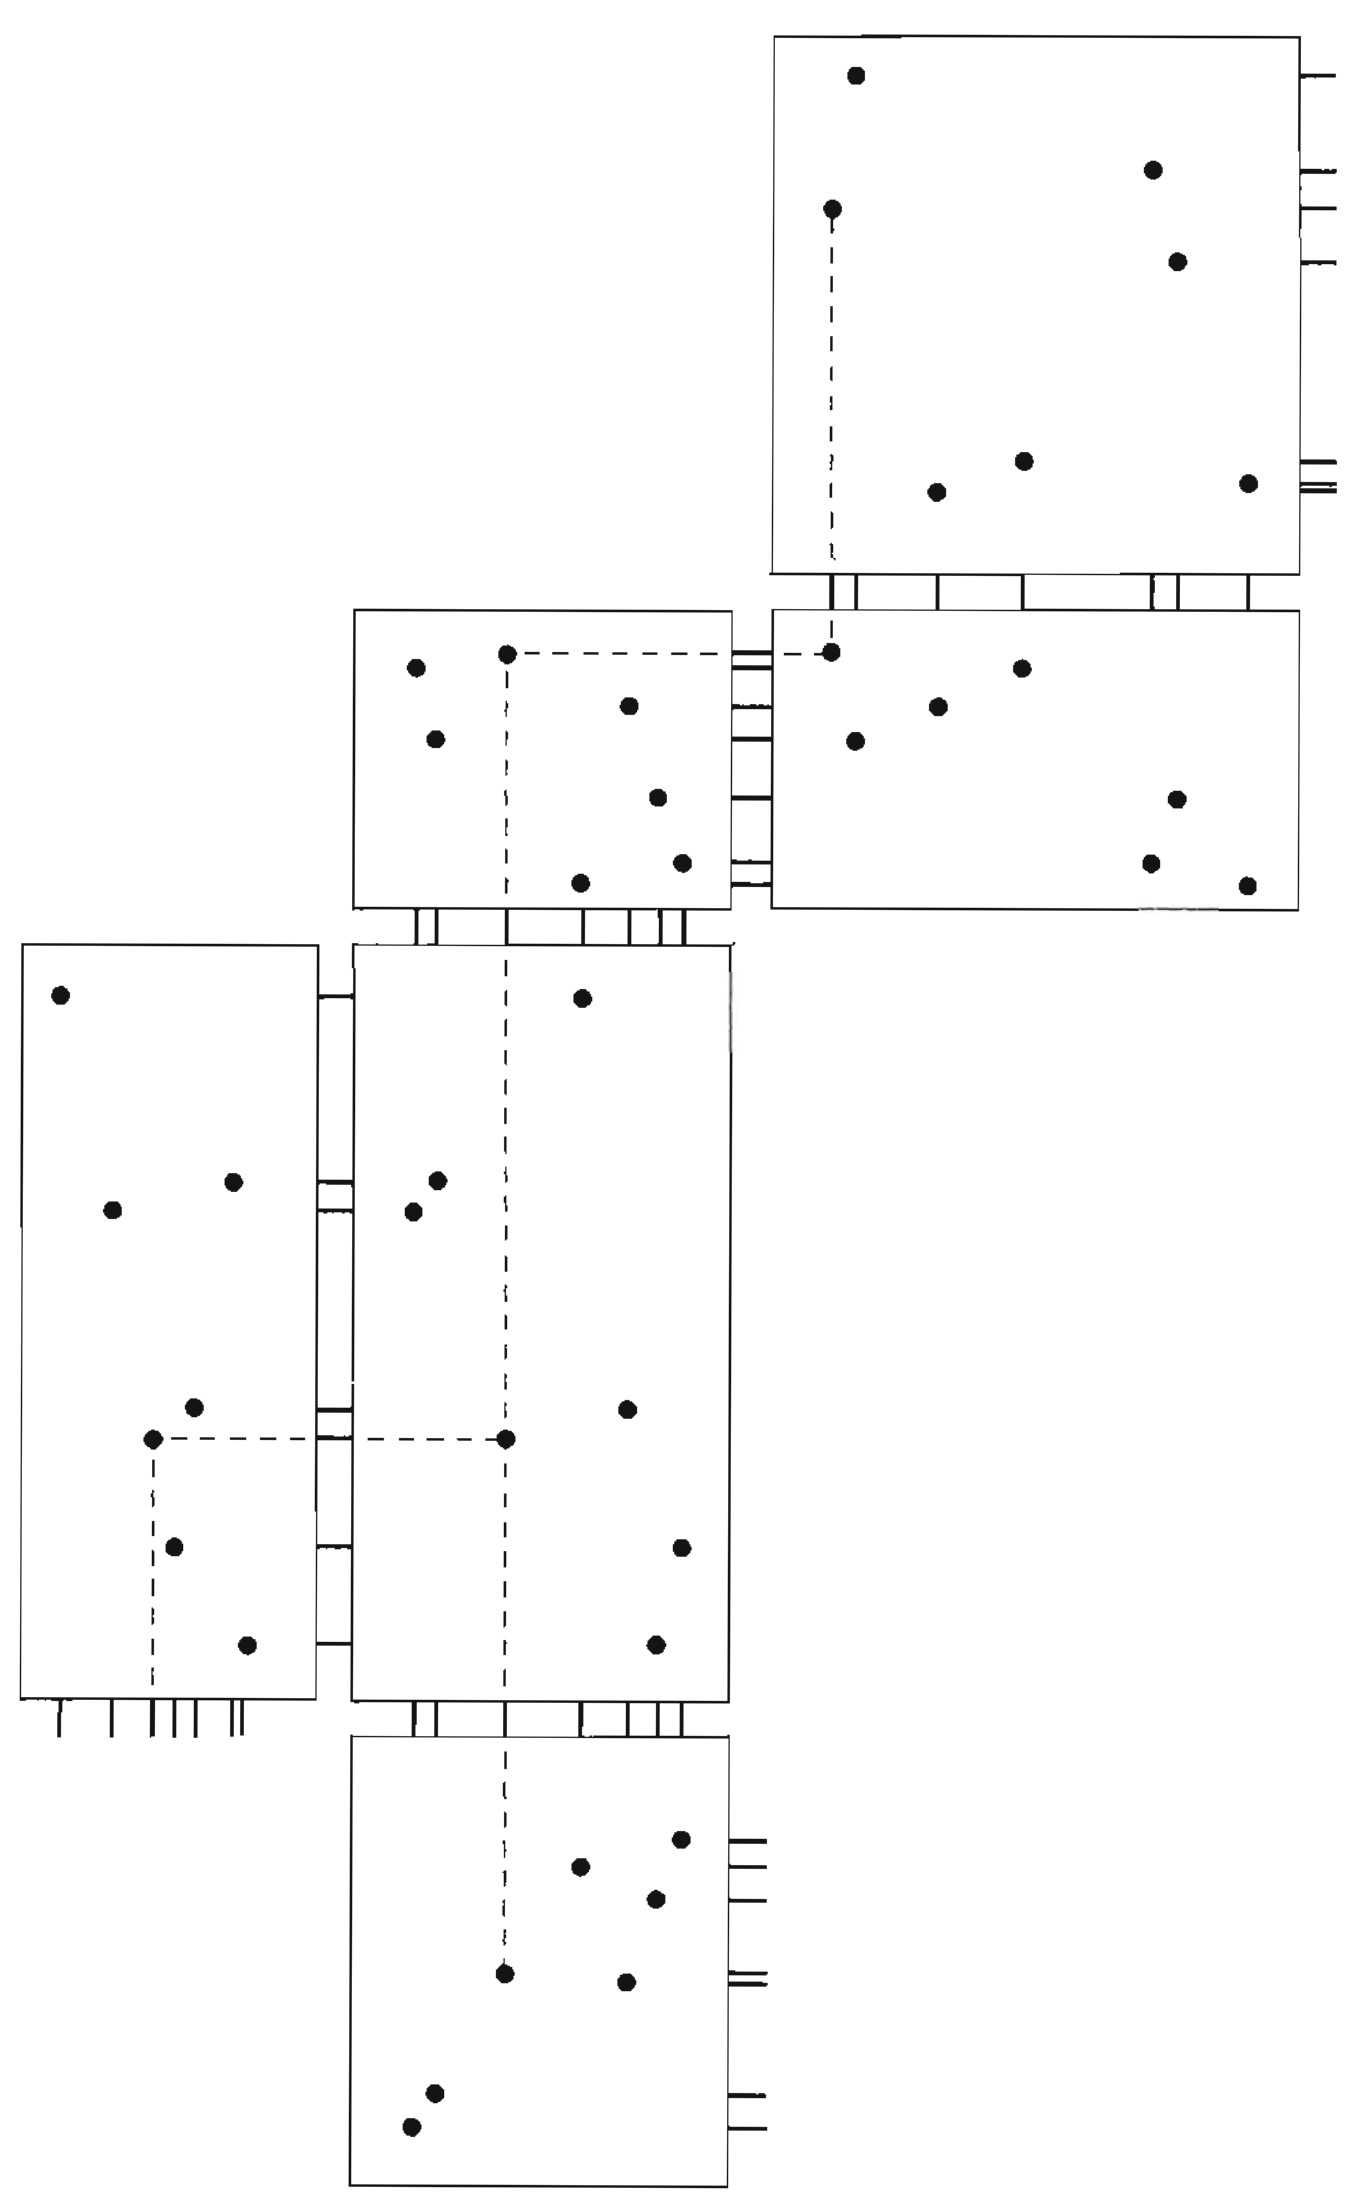
\includegraphics[width=0.35\textwidth]{images/rug_plot.png}
		\end{center}
	\end{figure}

\end{frame}

%% ========================= Data types ===================================
\section{Data Types Primer}

\begin{frame}{Data Types Map onto Chart Types!}{}
	In SMM635, we focus on the following data types:
	\begin{itemize}
		\item Nominal
		\item Ordinal
		\item Quantitative
		\item Temporal
	\end{itemize}
\end{frame}

\begin{frame}{Nominal Data}
	\small
	Nominal data — also called categorical data — consist of category names.

	\vspace{1em}

	With nominal data we can compare the equality of values: is value A the same or different than value B? (A = B), supporting statements like “A is equal to B” or “A is not equal to B”. In the dataset above, the country field is nominal.

	\vspace{1em}

	When visualizing nominal data we should readily perceive if values are
	the same or different: position, color hue (blue, red, green, etc.), and
	shape are all reasonable options. In contrast, using a size channel to
	encode nominal data might mislead us, suggesting rank-order or magnitude
	differences among values that do not exist!
\end{frame}

\begin{frame}{Ordinale Data}
	\small
	Ordinal data consist of values that have a specific ordering.

	\vspace{1em}

	With ordinal data we can compare the rank-ordering of values: does value A come
	before or after value B? (A < B), supporting statements like “A is less than B”
	or “A is greater than B”. In the dataset above, we can treat the year field as
	ordinal.

	\vspace{1em}

	When visualizing ordinal data, we should perceive a sense of rank-order.
	Position, size, or color value (brightness) might be appropriate, whereas color
	hue (which is not perceptually ordered) would be less appropriate.

\end{frame}

\begin{frame}{Quantitative Data}
	\small
	With quantitative data we can measure numerical differences among values. There are multiple sub-types of quantitative data:

	\vspace{1em}

	For interval data we can measure the distance (interval) between points: what is the distance to value A from value B? (A - B), supporting statements such as “A is 12 units away from B”.

	\vspace{1em}

	For ratio data the zero point is meaningful, so we can also measure proportions or scale factors: value A is what proportion of value B? (A / B), supporting statements such as “A is 10% of B” or “B is 7 times larger than A”.

	\vspace{1em}

	In the dataset above, year is a quantitative interval field (the value of year "zero" is subjective), whereas fertility and life_expect are quantitative ratio fields (zero is meaningful for calculating proportions). Vega-Lite represents quantitative data, but does not make a distinction between interval and ratio types.

	\vspace{1em}

	Quantitative values can be visualized using position, size, or color value, among other channels. An axis with a zero baseline is essential for proportional comparisons of ratio values, but can be safely omitted for interval comparisons.
\end{frame}

\begin{frame}{Temporal Data}

	\small

	Temporal values measure time points or intervals. This type is a special case of quantitative values (timestamps) with rich semantics and conventions (i.e., the Gregorian calendar).

	\vspace{1em}

	Example temporal values include date strings such as “2019-01-04” and “Jan 04 2019”, as well as standardized date-times such as the ISO date-time format: “2019-01-04T17:50:35.643Z”. There are no temporal values in our global development dataset above, as the year field is encoded as an integer.

	\vspace{1em}

	The temporal type in Vega-Lite supports reasoning about time units (year, month, day, hour, etc.), and provides methods for requesting specific time intervals. For more details about temporal data in Vega-Lite, see the TimeUnit documentation.

\end{frame}




% ========================== Session 3 wrap up =============================
\section{Session \#3 Wrap Up}

\begin{frame}{}{}
	\LARGE \centering Time to wrap up!
\end{frame}

% =========================== Bibliography =================================
\begin{frame}
	\frametitle{References}
	\printbibliography
\end{frame}

\end{document}
